
\section{Results}
\label{sec:experiments}


We evaluate \genco against classical and state-of-the-art neural solvers for power flow (PF) in \cref{subsec:pf}, optimal power flow (OPF) in \cref{subsec:opf}, and state estimation (SE) in \cref{subsec:SE}. We then study runtime and accuracy scaling with grid size and compare against classical AC and DC PF/OPF solvers in \cref{subsec:scaling}. Next, we assess generalization to topology perturbations, out-of-distribution operating conditions, and unseen grids in \cref{subsec:generalization}. Finally, we validate \genco on real SCADA data from the Hydro-Québec grid in \cref{subsec:hq1200}.

Throughout this section, we consider three \genco variants that differ only in their hidden dimension $H$, which determines the size of the input representations after projection (\cref{eq:input_proj}) and the latent space (\cref{eq:transformer}): \genco Base ($H=48$), Small ($H=24$), and Tiny ($H=12$), with 20.1M, 5.0M, and 1.3M parameters, respectively. All other architectural components are kept identical across variants. Unless stated otherwise, ``\genco'' refers to \genco Base.



\subsection{Power Flow}
\label{subsec:pf}

We evaluate \genco on Power Flow (PF) using PF$\Delta$~\cite{NEURIPS2025_d000ef56}, a benchmark of 12 tasks designed to assess neural PF solvers under varying topologies, data regimes, and operating conditions. We compare \genco against CANOS-PF (adapted from~\cite{piloto2024}), GNS-S~\cite{DONON2020106547}, and PFNet~\cite{lin2024powerflownet}, on the subset of tasks listed in \cref{tab:tasks-summary}, for which results on the IEEE 118-bus system were reported by the authors. Extensive comparisons against classical AC and DC solvers are presented in \cref{subsec:scaling}, as \pfdelta does not provide DC-PF solutions nor classical solver runtimes. CANOS-PF is a soft-constrained supervised model trained with a combination of an $\ell_2$ loss to precomputed AC power flow solutions and a penalty on power-balance residuals. PFNet is a purely supervised model trained with an $\ell_2$ loss on precomputed AC power flow solutions. GNS-S is a self-supervised method that iteratively minimizes power-balance violations through residual-based updates of nodal features.\\


\begin{table}
\centering
\small
\renewcommand{\arraystretch}{1.0}
\begin{tabularx}{\linewidth}{lX}
\toprule
\textbf{Task} & \textbf{Training setup} \\
\midrule
\multicolumn{2}{l}{\textbf{Generalization to topology perturbations}} \\
\midrule
1.1 & Train on (N) only. \\
1.2 & Train on (N) and (N{-}1). \\
1.3 & Train on (N), (N{-}1), and (N{-}2). \\
\midrule
\multicolumn{2}{l}{\textbf{Data efficiency}} \\
\midrule
2.1 & Baseline setting (same as 1.3; 54k training samples). \\
2.2 & \textit{Skipped; no results reported by the authors.} \\
2.3 & Same training composition as 2.1, with $3\times$ less training data (18k samples). \\
\midrule
\multicolumn{2}{l}{\textbf{Generalization to different grid sizes}} \\
\midrule
3.1 & Train on IEEE 118; evaluate on the unseen IEEE 57 and GOC 500 grids. \\
\midrule
\multicolumn{2}{l}{\textbf{Training on challenging PF cases}} \\
\midrule
4.1 & Train on 90\% feasible and 10\% C2I samples. \\
4.2 & Train on 50\% feasible, 10\% C2I, and 40\% approaching-infeasibility samples. \\
4.3 & Train on 20\% C2I and 80\% approaching-infeasibility samples only. \\
\bottomrule
\end{tabularx}
\caption{PF$\Delta$ tasks evaluated in this work. The tasks assess (i) generalization to topology perturbations (Tasks 1.x), (ii) data efficiency (Tasks 2.x), (iii) generalization to different grid sizes (Task 3.1), and (iv) the effect of training on challenging PF cases (Tasks 4.x). Each task trains a separate neural solver on the IEEE 118-bus system and is evaluated on (N), (N{-}1), (N{-}2), and close-to-infeasible (C2I) test cases for IEEE 118, except Task 3.1, which additionally evaluates on the unseen IEEE 57- and GOC 500-bus systems. Tasks 4.1--4.3 vary the composition of the training set by progressively replacing feasible samples with C2I and approaching-infeasibility samples. C2I and approaching-infeasibility samples correspond to operating points at and immediately preceding the steady-state stability limit, respectively.}
\label{tab:tasks-summary}
\end{table}





\begin{figure*} \centering 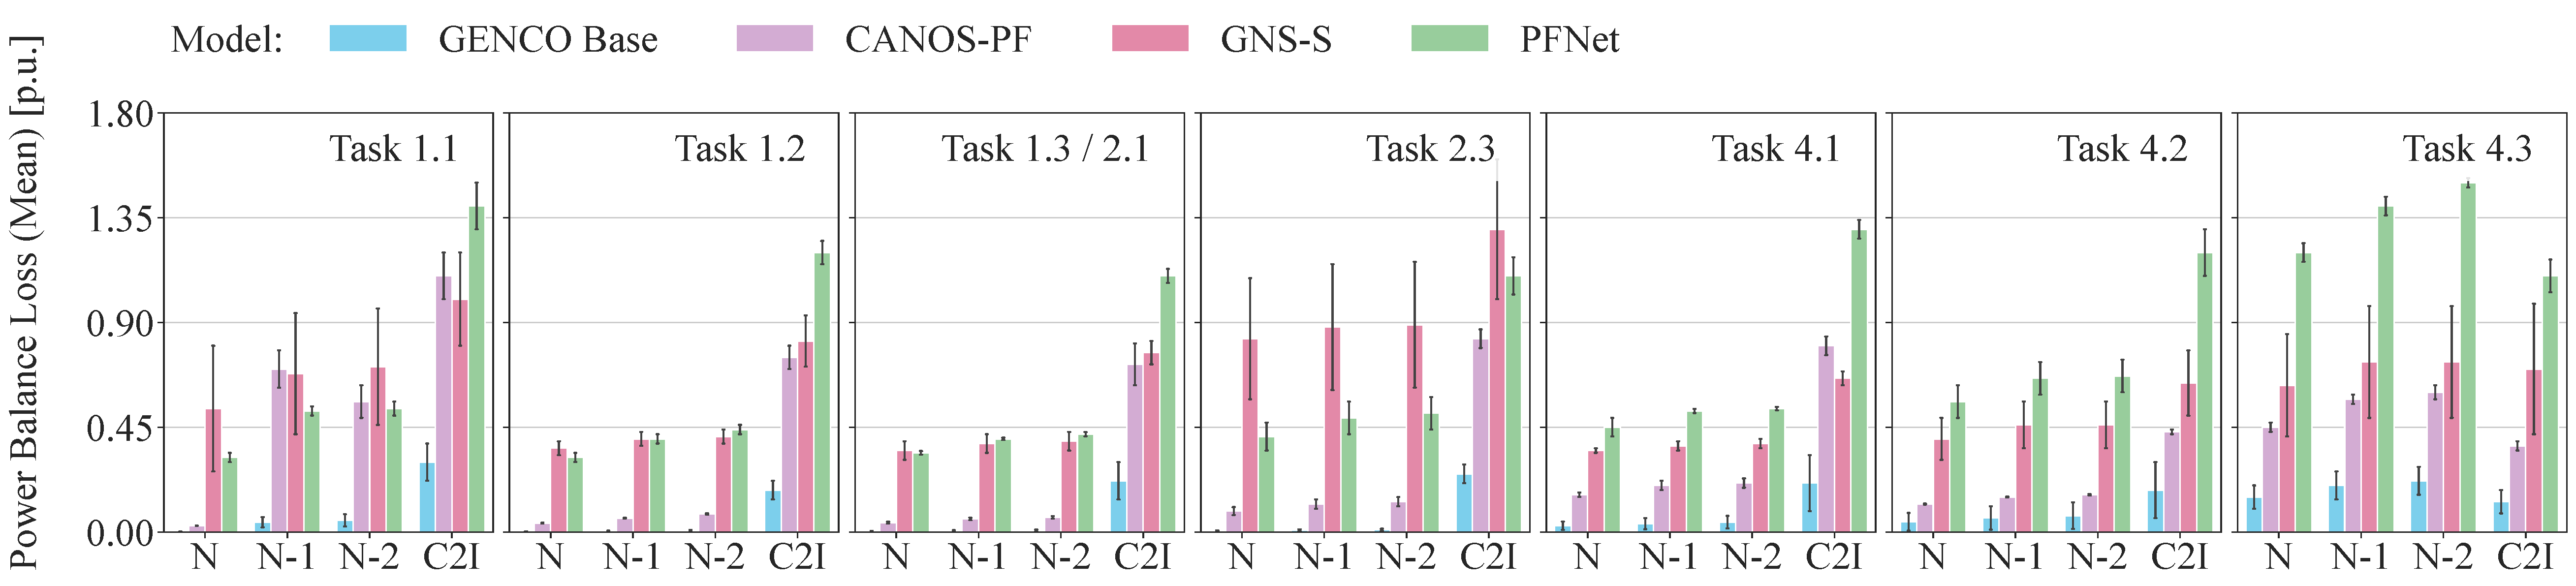
\includegraphics[width=\linewidth]{figures/pf_delta/pbl_all_rows_mean.pdf} 
\caption{Mean power-balance loss (averaged across all buses of all samples) for \genco, CANOS-PF, GNS-S, and PFNet across PF$\Delta$ tasks on the IEEE 118-bus system. Error bars in the figure correspond to the standard deviation over three seeds. C2I denotes close-to-infeasible cases at the steady-state stability limit, where classical solvers face challenges~\cite{NEURIPS2025_d000ef56}.}
\label{fig:mean-pb} \end{figure*}



We report mean power-balance loss as in~\cite{NEURIPS2025_d000ef56}, which is computed for each bus $k$ as the $\ell_2$ norm of the nodal power-balance residuals (defined in \cref{eq:PBRes}), i.e., $
\|\mathrm{PBRes}_k\|_2
=
\sqrt{\mathrm{PBRes}_{P,k}^2 + \mathrm{PBRes}_{Q,k}^2},
$
and averaged over all buses across all PF samples within a given test set, with values expressed in p.u. on a 100 MVA base, i.e., \(x_{\mathrm{p.u.}} = x / S_{\mathrm{base}}\), where \(S_{\mathrm{base}} = 100\,\mathrm{MVA}\) is the power base.\\

We report \genco's performance for all tasks except Task 3.1 (\cref{table:all-cases-mean}) in \cref{fig:mean-pb}. The results indicate that \genco achieves substantially lower errors and variance than all baselines across all tasks and topology variants. We complement the figure and additionally provide a relative measure of error magnitude, expressing the mean power-balance loss as a percentage of the mean bus apparent power injection\footnote{For a bus $k$, the apparent power is $|S_k| = \sqrt{P_{\mathrm{bus},k}^2 + Q_{\mathrm{bus},k}^2}$.}. In the baseline setting, where \genco is trained on (N), (N{-}1), and (N{-}2) topologies and evaluated on the corresponding test sets (Tasks 1.3/2.1), the loss amounts to only 0.28\%, 0.53\%, and 0.69\% of the mean apparent power under (N), (N{-}1), and (N{-}2) conditions, respectively (with mean bus apparent powers of 0.95, 0.87, and 0.86 p.u.). Among the baselines, only CANOS-PF remains within the single-digit percentage range (4.2\%, 6.4\%, and 7.3\%), whereas all other methods exhibit errors corresponding to approximately 40--50\% of the mean apparent power, indicating substantial violations of power-balance constraints and very limited physical consistency for these solvers.\\

Examining individual task groups provides further insight into \genco's behavior: Tasks~1.1--1.3 show that adding (N{-}1) contingencies to the training set is sufficient for \genco to generalize to both (N{-}1) and (N{-}2) topologies with essentially no loss in accuracy compared to (N). Even training only on (N) topologies already yields strong performance. In contrast, the baseline solvers, particularly CANOS-PF, exhibit substantially larger residuals on (N{-}1) and (N{-}2) topologies when such perturbations are absent from the training set. Tasks~2.1 and~2.3 further demonstrate that \genco maintains low error when the training set is reduced by a factor of three, while keeping the training composition and test sets unchanged. While CANOS-PF experiences only a modest degradation, the error of GNS-S nearly doubles between Tasks~2.1 and~2.3. Task~4.1 indicates that replacing 10\% of feasible training samples with close-to-infeasible (C2I) samples provides only marginal improvements on C2I test cases while slightly degrading performance on the remaining datasets compared to Tasks~1.3/2.1. Tasks~4.2 and~4.3 show that progressively increasing the proportion of challenging training samples, from 50\% to 100\%, further improves performance on C2I cases, particularly in terms of standard deviation, but comes at the expense of increased errors on the other datasets.\\

\cref{fig:max-pb} (Appendix) shows that \genco also achieves substantially lower \emph{maximum} power-balance errors than all baselines across (N), (N{-}1), and (N{-}2) topologies. On close-to-infeasible cases, however, GNS-S exhibits lower worst-case errors, potentially due to its self-supervised training objective, which may provide greater robustness to out-of-distribution operating conditions. Nevertheless, all methods exhibit very large worst-case residuals, often exceeding several times the mean apparent power\footnote{A more detailed analysis of the distribution of these residuals would be required to determine what fraction of test samples exhibit such large errors, which we leave for future work.}.\\






\input{figures/pf_delta/pf_delta_a_10}

Finally, Task~3.1 evaluates models trained on IEEE 118 on the unseen IEEE 57 and GOC 500 grids (\cref{table:all-cases-mean}). \genco achieves the lowest mean power-balance loss on both unseen grids, although all models suffer from substantial degradation under cross-grid evaluation. Relative to the mean apparent power averaged over (N), (N{-}1), and (N{-}2), \genco's mean error is approximately equal to the average apparent power on IEEE 57 and approximately 14$\times$ larger on GOC 500, while the baselines show even larger errors.\\ %(0.91, 0.49, and 0.63 p.u. for IEEE 118, IEEE 57, and GOC 500, respectively), 





\begin{boxH}
\paragraph{Takeaways.}
\begin{itemize}
\item When used to solve Power Flow, \genco achieves very low \emph{mean} power-balance residuals (\textless 1\% of the mean apparent power), lower than all state-of-the-art models on the PF$\Delta$ dataset.
\item It is more data-efficient and more robust to close-to-infeasible cases than competing methods.
\item All baseline models and \genco exhibit large worst-case errors and degraded performance on unseen grids, with power-balance residuals reaching multiples of the mean apparent power in both cases, highlighting the need for more robust solvers and more sophisticated pretraining.\end{itemize}
\end{boxH}

\subsection{Optimal Power Flow}
\label{subsec:opf}

\input{figures/opf/opf_ola}


We evaluate \genco on the OPFData~\cite{lovett2024opfdatalargescaledatasetsac} benchmark against the Hybrid Heterogeneous Message Passing Neural Network (HH-MPNN) proposed in~\cite{arowolo2025}, which is the latest baseline available for this dataset at the time of writing. We use the dataset version containing N-1 topology perturbations and follow exactly the same train/validation/test splits as in \cite{arowolo2025}: 270,000 samples for training (90\%), 15,000 for validation (5\%), and 15,000 for testing (5\%). Experiments are conducted on six benchmark systems ranging from 14 to 2000 buses. All \genco experiments are repeated over three random seeds while keeping identical data splits to ensure a fair comparison with \cite{arowolo2025}, which only reports results for one seed.
\\\\

\cref{tab:opf_results} reports both optimality and feasibility metrics. Optimality gap (\%) is computed as the mean relative objective gap with respect to the IPOPT solution over the test set. Feasibility metrics report absolute mean constraint violations: branch angle-difference violations $\theta_{ij}$ are zero for all solvers and considered cases and are therefore omitted, apparent power flow limit violations $S_{ij}(+)$ and $S_{ij}(-)$ in MVA for both branch directions, active and reactive power-balance residuals $\mathrm{PBRes}_{P}$ and $\mathrm{PBRes}_{Q}$ in MW and MVar, respectively (\cref{eq:PBRes}), and reactive generation limit violations $Q_g$ in MVar. All violations are averaged over all buses and lines across all test-set instances.
\\\\
The results highlight a trade-off between optimality and feasibility. On the smaller 14- to 118-bus systems, both solvers achieve highly feasible and optimal solutions overall. Moreover, \genco shows consistently lower reactive power-balance residuals $\mathrm{PBRes}_{Q}$, often by one to two orders of magnitude compared to HH-MPNN.
\\\\
On larger systems (500- and 2000-bus systems), HH-MPNN typically achieves lower objective gaps, whereas \genco attains substantially smaller branch thermal and reactive power-balance violations. For example, on the 2000-bus system, HH-MPNN reaches a near-zero optimality gap (potentially due to reduced constraint satisfaction), while \genco reduces branch flow violations from approximately $2.8 \times 10^{-3}$ to $2.3 \times 10^{-5}$~MVA (averaged over both directions).
\\\\
\genco consistently achieves lower $\mathrm{PBRes}_{Q}$ residuals because reactive generation $Q_g$ is reconstructed analytically from the reactive power-balance equations using the decoded voltage state, rather than being predicted directly. This physics-based completion makes reactive power-balance residuals structurally zero at PV and reference buses. This design trades reactive power-balance feasibility against explicit enforcement of reactive generation limits. Unlike \cite{arowolo2025}, \genco does not project reconstructed $Q_g$ onto generator limits using sigmoid activations, which can lead to small $Q_g$ violations. However, these remain negligible in practice: the largest mean violation is below 0.036\% of the mean reactive power limits.
\\\\
Finally, in addition to achieving an extremely small optimality gap (0.3\% in the worst case), we provide context for the magnitude of the reported violations by normalizing inequality constraints by their mean limits and equality constraints by the corresponding mean net injections.\footnote{A more informative metric would normalize each violation by its constraint limit before averaging. However, these quantities are not reported in~\cite{arowolo2025}, and the variability in constraint limits (including very small bounds) can make such metrics sensitive to outliers. We therefore report mean violations relative to mean constraint limits for inequality constraints, and use mean mismatches for equality constraints, to provide a sense of scale. We leave a more complete analysis for future work.}. The largest mean thermal violation to mean thermal limit ratio is obtained for IEEE 118, where violations represent 0.0018\% of the mean limits (0.0556\% for HH-MPNN on the same case). For the power-balance mismatch relative to mean net active injection, the worst case for \genco is GOC 2000 with 0.176\% (0.082\% for HH-MPNN on IEEE 118). For reactive power-balance mismatch relative to mean net reactive injection, the worst case is IEEE 57, with 0.340\% (1.38\% for HH-MPNN on IEEE 57).\\





 %      dataset  available_partitions  sampled_partitions  mean_rate_a  mean_net_active_injection  mean_net_reactive_injection  mean_qg_max_upper_bound
 %  case14_ieee                  1500                  50   190.984954                  37.608090                     7.475750                25.479667
 %  case30_ieee                  1500                  50    81.501405                  17.642591                     4.766607                30.663312
 %  case57_ieee                  1500                  50   298.077878                  30.791514                     8.770591                88.962080
 % case118_ieee                  1500                  50   248.450877                  62.270168                    17.880290               147.298577
 %  case500_goc                  1500                  50   370.190396                  70.808837                    15.957078                95.224356
 % case2000_goc                  1500                  50   217.340042                  33.364938                     8.230189               121.774097


\begin{boxH}
\paragraph{Takeaways.}

\begin{itemize}

\item For Optimal Power Flow, evaluated on OPFData, \genco achieves \textbf{competitive optimality} (worst-case gap $\leq0.3\%$) while substantially improving feasibility, with all \textbf{mean normalized feasibility violations remaining below $0.35\%$} across all grids.
\end{itemize}
\end{boxH}

\subsection{State Estimation}
\label{subsec:SE}

We evaluate \genco on State Estimation (SE), the task of recovering bus voltage magnitudes and phase angles from noisy, incomplete, and corrupted measurements. Classical state estimators formulate SE as a nonlinear inverse problem, most commonly solved using Weighted Least Squares (WLS), which relies on an accurate grid model and a sufficiently informative (i.e. locally observable) measurement set. In contrast, \genco learns a direct mapping from measurements to grid states by combining data-driven priors with physics-informed corrections, as described in \cref{sec:model}. % Rather than explicitly solving the inverse problem at inference time, it leverages the distribution of operating conditions observed during training together with physics-based corrective updates. 
We first evaluate its robustness to sparse, noisy, and outlier-corrupted measurements, as well as cases where WLS fails to converge, before studying its resilience to inaccuracies in the underlying grid model caused by admittance parameter errors.


\paragraph{Experimental setup.} GENCO models are trained on datasets generated via \datakit, comprising roughly 250{,}000 scenarios per grid, with varying N-k topology perturbations ($k=5$ for IEEE 14/30/57 and $k=10$ for IEEE 118) and admittance perturbations, on the standard IEEE 14, 30, 57, and 118-bus systems. In the absence of standardized datasets and procedures for generating synthetic SCADA measurements, we define our measurement-generation protocol and evaluation settings as follows. We generate SCADA measurements from the true bus voltage magnitudes $V$, bus power injections $P_{\text{inj}}, Q_{\text{inj}}$, and branch flows $P_{\text{flow}}, Q_{\text{flow}}$ by applying three different types of perturbations; first, we randomly mask a fraction $p_{\text{mask}}$ of the available measurements to emulate limited measurement coverage, with the resulting number of measurements expressed as a multiple of the number of buses $|\mathcal{N}|$; second, we apply multiplicative Gaussian noise ($\sigma_V = 0.01$~p.u., $\sigma_{P,Q} = 0.02$~p.u.) to all measurements, independently perturbing each measured voltage magnitude, active/reactive power injection, and active/reactive branch flow; third, we create outliers by adding a bias of three standard deviations to a fraction $p_{\text{outlier}}$ of measurements. We consider arbitrary measurement locations, but do not enforce sensor placement according to power-system observability rules. To mitigate this simplification, we use measurement densities above typical observability requirements (at least $5|\mathcal{N}|$ measurements, compared to the commonly used $4|\mathcal{N}|$ rule of thumb\footnote{\url{https://pandapower.readthedocs.io/en/latest/estimation.html}}, and $3.2 \text{ to } 4.6|\mathcal{N}|$ measurements used by Hydro-Québec~\cite{4596318}) and report results only on scenarios that remain observable under WLS. Voltage angles are never measured. To train GENCO models, we use $p_{\text{mask}} = 0.2$ and $p_{\text{outlier}} = 0.1$ and minimize the loss shown in \cref{eq:loss}, with $\mathcal{L}_{\text{supervised}}$ being the mean $\ell_1$ norm between true and predicted bus and edge variables.


% 345 kV maps closest to HQ's 3XX (315 kV) tier — highest-redundancy tier below the 735 kV backbone, m/n ≈ 3.7–4.6.
% 138 kV maps closest to HQ's 1XX (120–161 kV) tier — the largest single tier by measurement count (1413), with moderate redundancy, m/n ≈ 3.2–4.0.
% https://ieeexplore.ieee.org/document/4596318

\paragraph{Baseline and evaluation.} We compare \genco against a Weighted Least Squares (WLS) baseline solved with the Gauss--Newton (GN) algorithm and outlier rejection, using the pandapower implementation~\cite{pandapower}. WLS receives the standard deviations of the measurements, giving it an advantage over \genco, which must implicitly infer measurement uncertainty from the training distribution. We evaluate each scenario using the bus-averaged mean absolute error. In rare under-determined scenarios, WLS can converge to a solution substantially different from the reference state while remaining consistent with the measurements, producing large errors that disproportionately affect the mean. We therefore use the median across scenarios of the bus-averaged mean absolute error as our primary metric, reducing the influence of such cases without requiring an arbitrary threshold to identify and exclude them. The baseline is evaluated only when the measurement-function Jacobian is full rank; comparisons are thus reported on that subset. Results for cases where the baseline does not converge are shown in \cref{fig:non-observable} in \cref{app:se}. \


\paragraph{Robustness to sparse, noisy, and outlier measurements.}
We first evaluate \genco against WLS with varying numbers of measurements and outlier rates in \cref{fig:base-case}. One GENCO model is trained for each grid and evaluated across all measurement densities and outlier levels. Overall, \genco reconstructs states more accurately than WLS on the small grids---its median voltage magnitude error is up to an order of magnitude lower on the IEEE 14- and 30-bus cases---with a degradation on the larger grids. %More importantly, while WLS fails to converge on 1--6\% of the cases, \genco always returns a solution.\\
\\



\begin{figure}
    \centering
    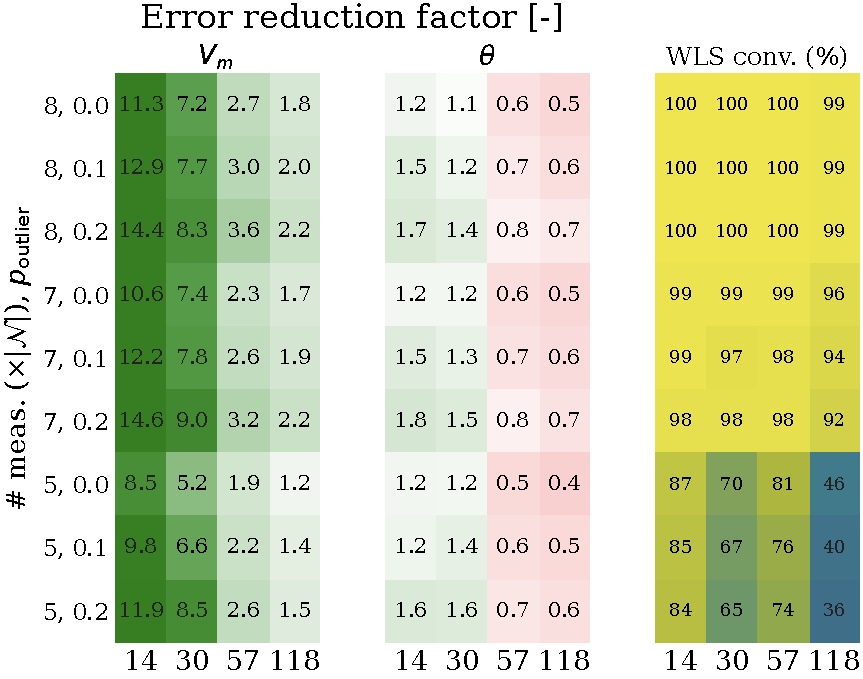
\includegraphics[width=\linewidth]{figures/se/base_case.pdf}
    \caption{State-estimation accuracy for varying numbers of noisy measurements and outlier probabilities. The first two panels show the error ratio of \genco relative to the WLS baseline (ratio of their median mean absolute errors) per variable: values above $1$ (green) indicate that \genco is more accurate, whereas values below $1$ (red) favor the baseline. The last column represents the percentage of scenarios in which the baseline converges; \genco always returns an estimate. Columns correspond to the IEEE 14-, 30-, 57-, and 118-bus grids.}
    \label{fig:base-case}
\end{figure}

As measurements become sparser and more corrupted, \genco remains robust, increasingly outperforming WLS on small grids and closing the gap with pandapower on larger grids. Note that the reported accuracy is computed only over scenarios where WLS converges, the number of which shrinks as measurements become sparser. \genco provides a complete estimator: unlike WLS, it returns an estimate even when the measurement configuration is insufficient for convergence. To assess the performance in cases where no WLS reference exists, \cref{fig:non-observable} reports the ratio between the errors of the non-converged and the converged subsets. Averaged across all sparsity levels, outlier rates, and grid-size settings, this ratio is $\approx 1.11$---a $\sim 10\%$ error increase on the cases where WLS yields no output at all. \genco thus degrades gracefully rather than failing abruptly, making it the more dependable estimator under marginal observability. Further improvements are required on larger grids, where \genco achieves the greatest gains in convergence robustness but falls short of WLS in accuracy.





\paragraph{Robustness to inaccurate grid parameters.}

While base grid parameters (e.g., admittance) are known to operators, they can drift throughout the day due to, e.g., temperature variations, which affect electrical resistance and the thermal expansion of transmission lines, resulting in line sag modulating the shunt capacitance. Consequently, the true grid parameters differ from the nominal parameters used by the state estimator. In \cref{fig:perturbation}, we evaluate \genco under grid parameter errors by perturbing the admittance with multiplicative factors sampled from a uniform distribution between $[1-\sigma_Y, 1+\sigma_Y]$. During training, measurements were consistent with the grid parameters, whereas during evaluation, the test set contains measurements that are generated using perturbed parameters, while the estimator receives the nominal admittance. Because \genco treats the grid physics as a soft prior rather than a hard constraint, it absorbs these discrepancies and keeps improving over the baseline as $\sigma_Y$ grows. In comparison, WLS enforces the now-incorrect model equations, causing the outlier-rejection procedure to incorrectly flag valid measurements and making non-convergence increasingly likely.\\


\begin{figure}
    \centering
    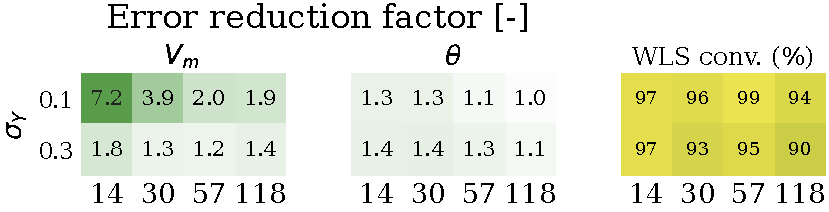
\includegraphics[width=\linewidth]{figures/se/unknown_perturbation.pdf}
    \caption{Robustness to inaccurate admittance parameters, evaluated across increasing admittance-noise levels $\sigma_Y$ (rows). The estimators are given only the base admittance matrix, before perturbation. The first two panels show the error ratio of \genco relative to the WLS baseline (ratio of median mean absolute errors) per state variable; values above $1$ (green) indicate that \genco is more accurate. The last panel depicts the convergence rate of the WLS solver; \genco always returns an estimate. Columns are the IEEE 14-, 30-, 57-, and 118-bus grids.} \label{fig:perturbation}
\end{figure}


By only adding an auxiliary decoder to the architecture discussed in \cref{sec:model}, \genco can simultaneously estimate bus states and grid parameters. We demonstrate this approach by perturbing the branch resistance/reactance ($R$, $X$) parameters with multiplicative uniform noise on $[1-\sigma', 1+\sigma']$ (half-width $\sigma'_R = \sigma'_X = 0.2$%, corresponding to an expected absolute relative deviation of $\sigma'/2 = 0.1$
) prior to inference. \genco successfully denoises the input parameters, achieving a $30$--$50\%$ reduction in noise magnitude across all tested IEEE grids. \\ %: mean relative errors on the predicted branch admittances drop consistently to a range of $0.05$--$0.07$.\\






\begin{boxH}
\paragraph{Takeaways.}
\begin{itemize}
\item SE is a task where \genco can surpass classical estimators under challenging measurement conditions. It is strongest exactly where WLS is limited by its reliance on an accurate grid model and sufficient observability:
\begin{itemize}
\item It achieves \textbf{better estimates than WLS under sparse and corrupted measurements}, although scaling this advantage to larger grids remains future work.
\item It \textbf{always returns an estimate}, maintaining good accuracy in scenarios where WLS fails to converge.
\item By treating the grid model as a soft prior rather than a hard constraint, it remains \textbf{robust to inaccurate grid parameters}.
\end{itemize}
\item The same architecture naturally extends to joint state and parameter estimation, recovering system states while denoising branch parameters.
\end{itemize}
\end{boxH}

\subsection{Runtime and Performance Scaling}
\label{subsec:scaling}


The promise of neural solvers is to reduce time-to-solution compared with classical methods for batched PF and OPF problems. We therefore evaluate solver runtime and residuals across batches of PF and OPF instances and grid sizes, reflecting realistic utility workloads where large collections of scenarios are repeatedly solved for applications such as planning, time-series forecasting, contingency analysis, and uncertainty quantification, rather than a single isolated operating point. Since the datasets used in \cref{subsec:pf} and~\ref{subsec:opf} do not include DC solutions, we use \datakit datasets, which provide solutions obtained with all classical AC-PF/AC-OPF and DC-PF/DC-OPF solvers implemented through PowerModels~\cite{powermodels}. This enables comparison against the PowerModels implementations of AC-PF (Newton--Raphson), AC-OPF (IPOPT with MUMPS), DC-PF, and DC-OPF\footnote{A fully controlled comparison of runtime and residuals with other neural solvers from the literature remains challenging because prior work uses different benchmarking protocols and heterogeneous hardware and inputs.}. All GENCO models are trained from scratch for each task and grid.

\subsubsection{Batch Runtime Analysis Methodology}

\begin{figure*}[t]
    \centering
    % Requires in the preamble:
    % \usepackage{graphicx}
    % \usepackage{tikz}
    % \usetikzlibrary{arrows.meta,positioning,fit,calc}
    \resizebox{\textwidth}{!}{%
    \begin{tikzpicture}[
        >=Latex,
        font=\large,
        node distance=5mm and 8mm,
        every node/.style={align=center},
        box/.style={
            draw,
            rounded corners,
            minimum width=1.3cm,
            minimum height=8mm,
            inner sep=3pt,
            fill=white
        },
        sidebox/.style={
            draw,
            rounded corners,
            minimum width=3.1cm,
            minimum height=8mm,
            inner sep=3pt,
            fill=white
        },
        titlebox/.style={
            draw,
            rounded corners,
            font=\large\bfseries,
            minimum width=1.3cm,
            minimum height=9mm,
            inner sep=3pt,
            fill=white
        },
        metricbox/.style={
            draw,
            rounded corners,
            minimum width=1.3cm,
            minimum height=10mm,
            inner sep=4pt,
            fill=white
        },
        flow/.style={-Latex, thick},
        note/.style={font=\normalsize, align=center},
        stage/.style={font=\large\bfseries, align=left}
    ]
    
    % Row titles
    \node[titlebox] (GENCOTitle) {\rotatebox{90}{\genco}};
    \node[titlebox, below=35mm of GENCOTitle]
(pmTitle) {\rotatebox{90}{\shortstack{Classical solver\\(PowerModels)}}};

    % \genco row
    \node[box, right=8mm of GENCOTitle] (gLoad) {Load model\\and compile};
    \node[box, right=of gLoad] (gPreload) {Preload \\input data \\into RAM};
    \node[box, right=of gPreload] (gWarmup) {Warmup};
    \node[box, right=10mm of gWarmup] (gLoop) {Repeated batched\\inference loop};
    \node[sidebox, above=7mm of gLoop] (gCpu) {32 CPU workers\\prepare batches};
    \node[box, right=of gLoop] (gTransfer) {Transfer \\batch\\to GPU};
    \node[box, right=of gTransfer] (gNorm) {Normalize \\inputs};
    \node[box, right=of gNorm] (gForward) {Model\\forward \\pass};
    \node[box, right=of gForward] (gInverse) {Inverse-norm.\\outputs};
    \node[metricbox, right=10mm of gInverse] (gMetric) {Reported metric:\\wall-clock time per\\solved instance};
    \node[note, below=3mm of gMetric] (gNote) {Batched GPU inference\\with background CPU batch preparation};
    
    % PowerModels row
    \node[box, right=8mm of pmTitle] (pPool) {Create\\worker pool};
    \node[box, right=of pPool] (pInit) {Initialize one Julia\\runtime per worker};
    \node[box, right=of pInit] (pCase) {Load base case into\\worker memory};
    % \node[box, right=of pCase] (pPrep) {For PF/DC-PF only:\\prepare OPF\\ setpoints once};
    \node[box, right=of pCase] (pWarmup) {Warmup solve\\per worker};
    \node[box, right=15mm of pWarmup] (pLoop) {Repeated\\solve loop};
    \node[sidebox, above=7mm of pLoop] (pSched) {Dynamic scheduling:\\next instance goes to\\first available worker};
    \node[box, right=of pLoop] (pSolve) {Each worker solves\\one instance at a time};
    \node[metricbox, right=10mm of pSolve] (pMetric) {Reported metric:\\wall-clock time per\\solved instance};
    \node[note, below=3mm of pMetric] (pNote) {Multi-process CPU solving\\with dynamic scheduling};
    
    % Flows
    \draw[flow] (gLoad) -- (gPreload);
    \draw[flow] (gPreload) -- (gWarmup);
    \draw[flow] (gWarmup) -- (gLoop);
    \draw[flow] (gLoop) -- (gTransfer);
    \draw[flow] (gTransfer) -- (gNorm);
    \draw[flow] (gNorm) -- (gForward);
    \draw[flow] (gForward) -- (gInverse);
    \draw[flow] (gInverse) -- (gMetric);
    \draw[flow] (gCpu.south) -- (gLoop.north);
    
    \draw[flow] (pPool) -- (pInit);
    \draw[flow] (pInit) -- (pCase);
    % \draw[flow] (pCase) -- (pPrep);
    \draw[flow] (pCase) -- (pWarmup);
    \draw[flow] (pWarmup) -- (pLoop);
    \draw[flow] (pLoop) -- (pSolve);
    \draw[flow] (pSolve) -- (pMetric);
    \draw[flow] (pSched.south) -- (pLoop.north);
    
    % Excluded and included timing groups
    \node[draw, dashed, rounded corners, inner sep=6pt, fit=(gLoad)(gPreload)(gWarmup)] (gExcluded) {};
    \node[stage, above left=0mm and -1mm of gExcluded.north west, anchor=south west] {Excluded from timing};
    \node[draw, rounded corners, inner sep=6pt, fit=(gLoop)(gCpu)(gTransfer)(gNorm)(gForward)(gInverse)] (gIncluded) {};
    \node[stage, above left=0mm and -1mm of gIncluded.north west, anchor=south west] {Included in timing: \\Time to solve a fixed number of PF/OPF instances};
    
    \node[draw, dashed, rounded corners, inner sep=6pt, fit=(pPool)(pInit)(pCase)(pWarmup)] (pExcluded) {};
    \node[stage, above left=0mm and -1mm of pExcluded.north west, anchor=south west] {Excluded from timing};
    \node[draw, rounded corners, inner sep=6pt, fit=(pLoop)(pSched)(pSolve)] (pIncluded) {};
    \node[stage, above left=0mm and -1mm of pIncluded.north west, anchor=south west] {Included in timing: \\Time to solve a fixed number of PF/OPF instances};
    
    \end{tikzpicture}
    }
    \caption{Benchmark pipelines used for runtime comparison. Top: for \genco, we measure steady-state throughput of batched GPU inference after model setup, sample preloading, and warmup. Bottom: for classical solvers, we measure steady-state throughput of a dynamically scheduled multi-process CPU solver pool after worker initialization, case loading, and warmup. Both report wall-clock time per solved instance, but they exploit parallelism differently: \genco through batching on a single GPU, and the classical solvers through multiple independent worker processes.}
    \label{fig:benchmark_pipeline_diagram}
    \end{figure*}
    

To ensure a fair runtime comparison, we evaluate both solvers under their best achievable throughput configurations while controlling for factors unrelated to the solution process. In particular, four aspects need to be carefully designed: (i) the evaluation metric and parallelization mode, (ii) benchmark scenarios, (iii) timing scope, and (iv) compute hardware. \Cref{fig:benchmark_pipeline_diagram} summarizes the benchmark pipelines and timing boundaries; complete implementation details and parameters are provided in \cref{app:runtime_details}.

\paragraph{Evaluation metric and parallelization mode.}
We measure the \emph{amortized per-instance runtime}, defined as the total wall-clock time required to solve a large batch of PF/OPF instances divided by the number of solved instances. 
Neural and classical approaches exploit different forms of parallelism: \genco performs batched GPU inference, whereas the classical solvers implemented through PowerModels exploit CPU parallelism through multiple workers, with each worker solving instances sequentially on a single CPU core.
We thus carefully design our experiments so that both solver classes are evaluated at their maximum throughput: For each grid and solver, we select the batch size or number of workers that minimizes our runtime metric, ensuring that neither approach is evaluated below its optimal throughput configuration\footnote{Note that previous runtime benchmarks of neural solvers evaluated classical baselines without the CPU parallelism used in our experiments, which can favor neural solvers in runtime comparisons~\cite{NEURIPS2025_d000ef56, arowolo2025, piloto2024}.}.


\paragraph{Benchmark scenarios.}
% We focus on batched scenario analysis in which scenarios are generated in memory by perturbing a given base network. This reflects use cases such as time-series analysis, contingency screening, and sensitivity studies, where many related grid states are evaluated around a reference operating point. A challenge is that classical solver runtime depends on scenario difficulty, through, e.g., the number of iterations required for convergence, whereas neural solvers' inference is largely insensitive to scenario difficulty. We therefore repeatedly use the base case of each grid, which provides a representative reference operating point while controlling for scenario difficulty. This avoids substantially harder or non-convergent scenarios that could introduce scenario-dependent runtime variation for classical solvers. For failed solves, runtime would additionally depend on the maximum number of iterations. In addition, this makes the experiment more reproducible by eliminating the need to choose a scenario distribution. To complement this analysis, \cref{app:runtime_details} reports a second protocol for heterogeneous grid snapshots, such as archived scenarios or externally generated datasets, where each scenario is an independent input loaded from disk. This experiment evaluates a distinct use case in which data loading is part of the workload, complementing the main benchmark based on in-memory perturbations around a base operating point.\\
We focus on batched scenario analysis in which evaluated scenarios are typically obtained in memory by applying small changes (e.g., to topology or load) to a given base network, reflecting use cases such as time-series analysis, contingency screening, and sensitivity studies. A challenge is that classical solver runtime depends on scenario difficulty, through, e.g., the number of iterations required for convergence, whereas neural solvers' inference is largely insensitive to scenario difficulty. The runtime of classical solvers is also affected by failed solves, for which the runtime depends on the maximum iteration limit. To avoid favoring neural solvers through harder or non-convergent scenarios, and to make the experiment reproducible without choosing a scenario distribution, the timed main protocol repeatedly solves the fixed base case of each grid (already resident in memory). To complement this analysis, \cref{app:runtime_details} reports a second \emph{from-disk} protocol for heterogeneous grid snapshots, such as archived scenarios or externally generated scenarios, where each scenario is an independent \datakit scenario loaded from disk and data loading is part of the measured workload.\\


To ensure a reliable throughput estimate, all solvers are evaluated on a sufficiently large number of repeated cases to reduce measurement noise from non-deterministic hardware effects, such as OS scheduling, CPU frequency fluctuations, and background processes. The number of repetitions is chosen to provide stable timing measurements (with at least 20~s of total solve time in the best-performing configuration) while remaining computationally tractable, as this evaluation is repeated across batch sizes and CPU worker counts to identify the optimal configuration.


\paragraph{Timing scope.}
We measure steady-state solver throughput rather than end-to-end pipeline latency, excluding one-time infrastructure overheads unrelated to the repeated PF/OPF solution process. These overheads depend on implementation choices and system factors rather than the numerical efficiency of the solver.
Thus, for a fair comparison, we exclude some components for both neural and classical solvers, i.e., worker initialization (PowerModels solver workers and \genco data-loading workers), compilation and warmup (Julia compilation and model compilation), and initial disk-to-RAM loading of the base network. 




\paragraph{Compute hardware.}
A fair comparison requires CPU and GPU hardware from the same node generation and performance class\footnote{Energy consumption and hardware cost are also relevant metrics but are difficult to compare fairly.}. In this study, we benchmark the solvers using two high-end devices, an AMD EPYC 9634 CPU with 84 cores and an NVIDIA H100 SXM5 GPU with 80GB HBM3 memory, both with a node size of 5nm and release date of late 2022. \\




\subsubsection{PF Scaling with Grid Size: Runtime and Accuracy}
 
We first study the trade-off between runtime and accuracy of the different solvers for PF.\\


\begin{figure}
    \centering
    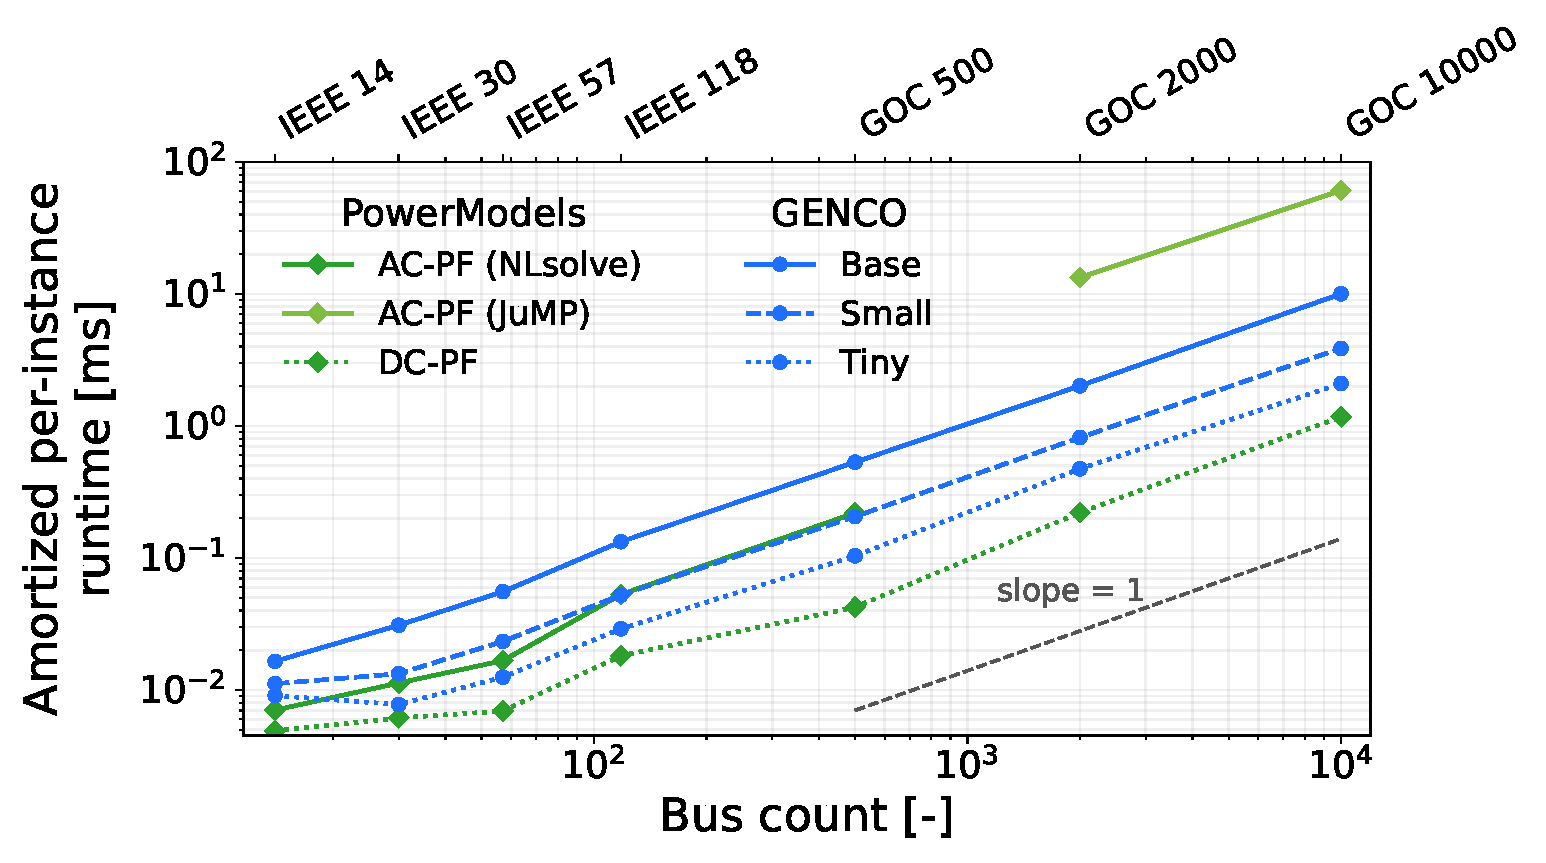
\includegraphics[width=\linewidth]{figures/runtime_analysis/runtime_comparison_from_raw_pf.pdf}
    \caption{Amortized per-instance runtime versus grid size for \genco and PowerModels AC-PF and DC-PF at the best batch size or worker count. Scaling exponents fitted on the four largest grids (two for AC-PF) are comparable across all methods, ranging from 0.94 to 0.97.}
    \label{fig:gridsize_runtime_pf}
\end{figure}


\begin{figure}
    \centering
    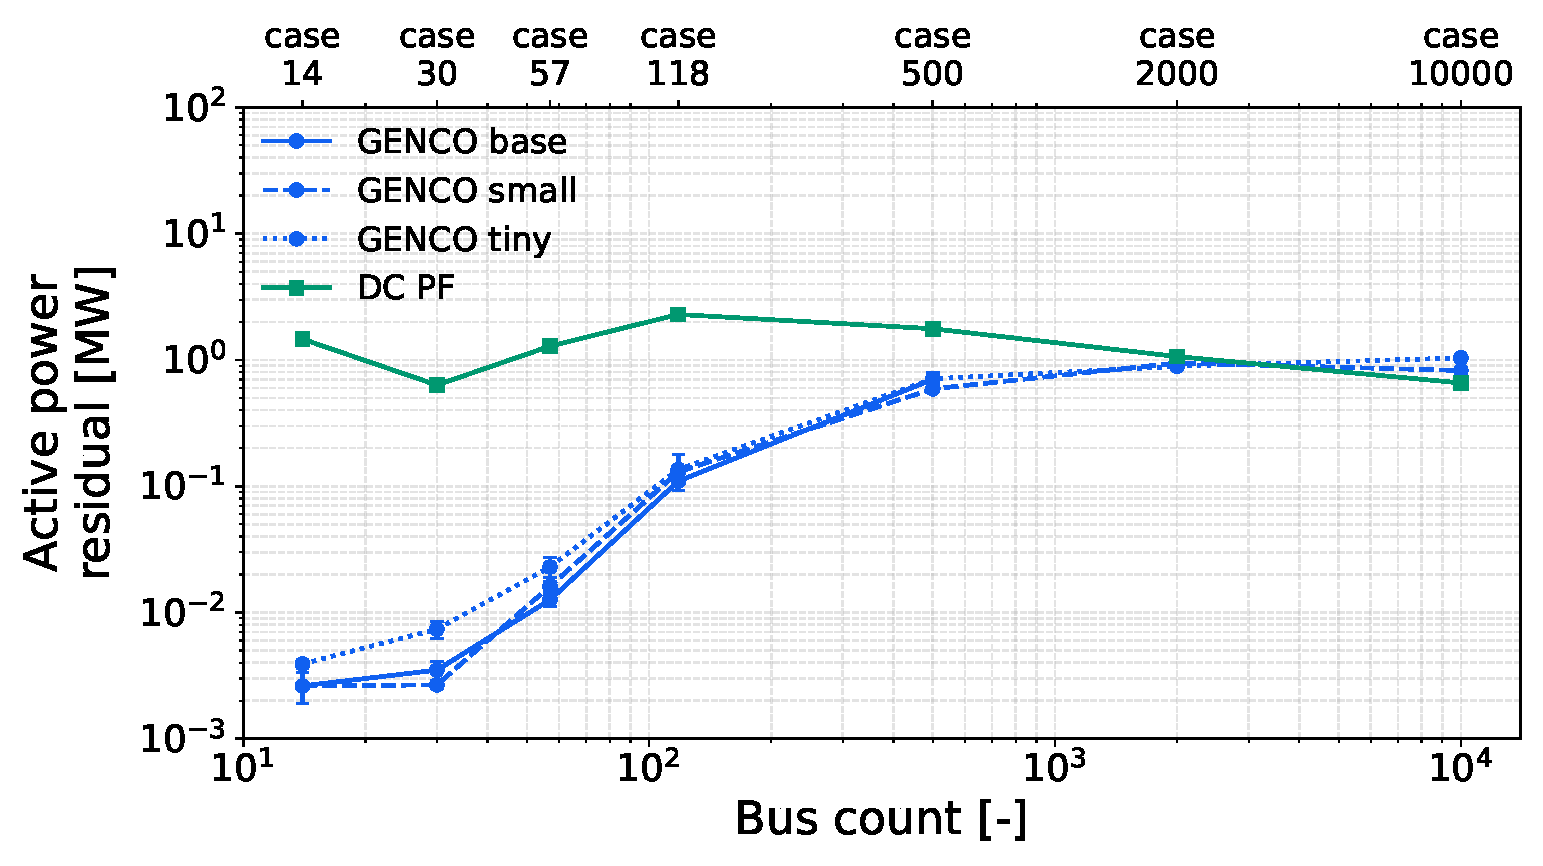
\includegraphics[width=1\linewidth]{figures/runtime_analysis/grid_scaling_active_residuals_pf.pdf}
    \caption{Mean active power-balance residuals versus grid size for \genco and PowerModels DC-PF.}
   \label{fig:gridsize_vs_residuals_pf}
\end{figure}


\paragraph{Runtime and accuracy for different grid sizes.}
The amortized per-instance runtime of \genco, AC-PF, and DC-PF as a function of bus count at the optimal batch size (\genco) or worker count (for the PowerModels-based classical solvers) is depicted in \cref{fig:gridsize_runtime_pf}. The runtime of all \genco versions (Base, Small, and Tiny) scales close to linear with grid size. For AC-PF, we selected the fastest converging solver available in PowerModels: the NLsolve-based solver for grids up to 500 buses and the JuMP-based solver for larger grids, as indicated by the disconnected lines. For large grids, the slopes of all solvers are similar, while for small networks AC-PF and DC-PF runtimes are nearly constant as multiprocessing overhead dominates. Active power-balance residuals are shown in \cref{fig:gridsize_vs_residuals_pf}. PowerModels AC-PF residuals ($10^{-11}$--$10^{-8}$~MW) are omitted for readability, while DC-PF remains near 1~MW. \genco increases from about $10^{-3}$~MW on the smallest IEEE grids to about 1~MW on GOC~2,000 and GOC~10,000. Its residuals are substantially lower than for DC-PF through GOC~500, slightly lower on GOC~2,000, and comparable to or slightly above for GOC~10,000, where Small outperforms Tiny; Base is evaluated only through GOC~500.\\





\paragraph{\genco's utility for PF.} \cref{tab:pf_selected_genco_tradeoff} summarizes the PF speed--accuracy trade-off, focusing on \genco Tiny because it provides the highest throughput while retaining useful solution accuracy: For a learned PF surrogate to be compelling, it must first provide a meaningful speedup over AC-PF, whose solutions are more accurate; modest gains may not offset the cost of training, maintaining, and deploying the neural solver. This criterion is not met on the small grids up to 500 buses, and the approximately $2\times$ speedup on GOC~500 remains marginal. In contrast, \genco Tiny is approximately $28$--$29\times$ faster than AC-PF on GOC~2,000 and GOC~10,000, making the learned approach increasingly attractive at scale. On these grids, \genco provides a good alternative to DC-PF: unlike DC-PF, it predicts a complete AC state, including voltage magnitudes and reactive generation, and therefore supports downstream voltage- and reactive-power-based analyses. For this reason, \genco can remain useful even when it is moderately slower or has slightly larger active power-balance residuals than DC-PF. On GOC~2,000 and GOC~10,000, it achieves similar residuals while being approximately $2\times$ slower than DC-PF. Overall, \genco Tiny is compelling for large-scale PF, where it substantially outperforms AC-PF and provides a complete AC state at a modest slowdown relative to DC-PF; on grids through GOC~500, AC-PF remains preferable.

\begin{table}
\centering
\scriptsize
\setlength{\tabcolsep}{3pt}
\renewcommand{\arraystretch}{1.1}
\begin{tabular}{@{}l c c c >{\raggedright\arraybackslash}p{0.35\linewidth}@{}}
\toprule
Grid
& \shortstack{Speedup\\vs AC-PF}
& \shortstack{DC-PF/\genco\\residual}
& \shortstack{Speedup\\vs DC-PF}
& Utility \\
\midrule
  14 & $0.8\times$ & $374.0\times$ & $0.5\times$ & 
  \multirow{5}{=}{None. Slower than AC-PF, which should be preferred since it provides more accurate solutions.} \\
  30 & $1.5\times$ & $85.8\times$ & $0.8\times$ &  \\
  57 & $1.3\times$ & $56.1\times$ & $0.6\times$ &  \\
 118 & $1.8\times$ & $16.9\times$ & $0.6\times$ &  \\
 500 & $2.1\times$ & $2.49\times$ & $0.4\times$ &  \\
\midrule
2000 & $28.2\times$ & $1.19\times$ & $0.5\times$ &
\multirow{6}{=}{\raggedright
Much faster than AC-PF; provides complete solutions with near-DC-PF active power-balance residuals at only 2× the runtime of DC-PF.} \\
10000 & $29.1\times$ & $0.63\times$ & $0.6\times$ & \\
& & & & \\
& & & & \\
& & & & \\
& & & & \\
\bottomrule
\end{tabular}
\caption{Scaling performance summary for \genco on Power Flow. Speedups $>$1 mean faster; the Utility column summarizes the recommended use of \genco relative to AC-PF and DC-PF for each grid-size. Results are for \genco Tiny for all grid sizes as it provides the best speedups and reasonable performance.}
\label{tab:pf_selected_genco_tradeoff}
\end{table}

\subsubsection{OPF Scaling with Grid Size: Runtime and Accuracy}

The amortized per-instance runtime as a function of grid size for AC-OPF, DC-OPF, and \genco is shown in \cref{fig:gridsize_runtime_opf}. The runtime values for \genco are independent of the task and thus identical to \cref{fig:gridsize_runtime_pf}. However, OPF is substantially harder to solve for classical solvers, resulting in a runtime advantage for \genco across all grid sizes.\\

% For a sequential comparison with CANOS, which reports per-sample solve times without parallelization, we use the best mean per-worker runtime from setup s2, which includes scenario parsing and solving.%
% % s2 best mean_pf_runtime_s worker counts: AC-OPF p=24 (GOC 500), p=24 (GOC 2000), p=40 (GOC 10000); DC-OPF p=24 (GOC 500), p=24 (GOC 2000), p=24 (GOC 10000).
% For AC-OPF, this yields 1.04~s for GOC~500, 6.65~s for GOC~2,000, and 51.5~s for GOC~10,000, compared to 6.49~s, 83.78~s, and 869.54~s, respectively, reported for AC-IPOPT before power-flow post-processing in CANOS~\cite{piloto2024}. These runtimes are approximately $6\times$ to $17\times$ lower. Our corresponding DC-OPF times (0.097~s, 0.457~s, and 3.19~s) are likewise about $9\times$ to $16\times$ lower than the CANOS DC-IPOPT before-power-flow runtimes (1.3~s, 4.27~s, and 50~s).




\begin{figure}
    \centering
    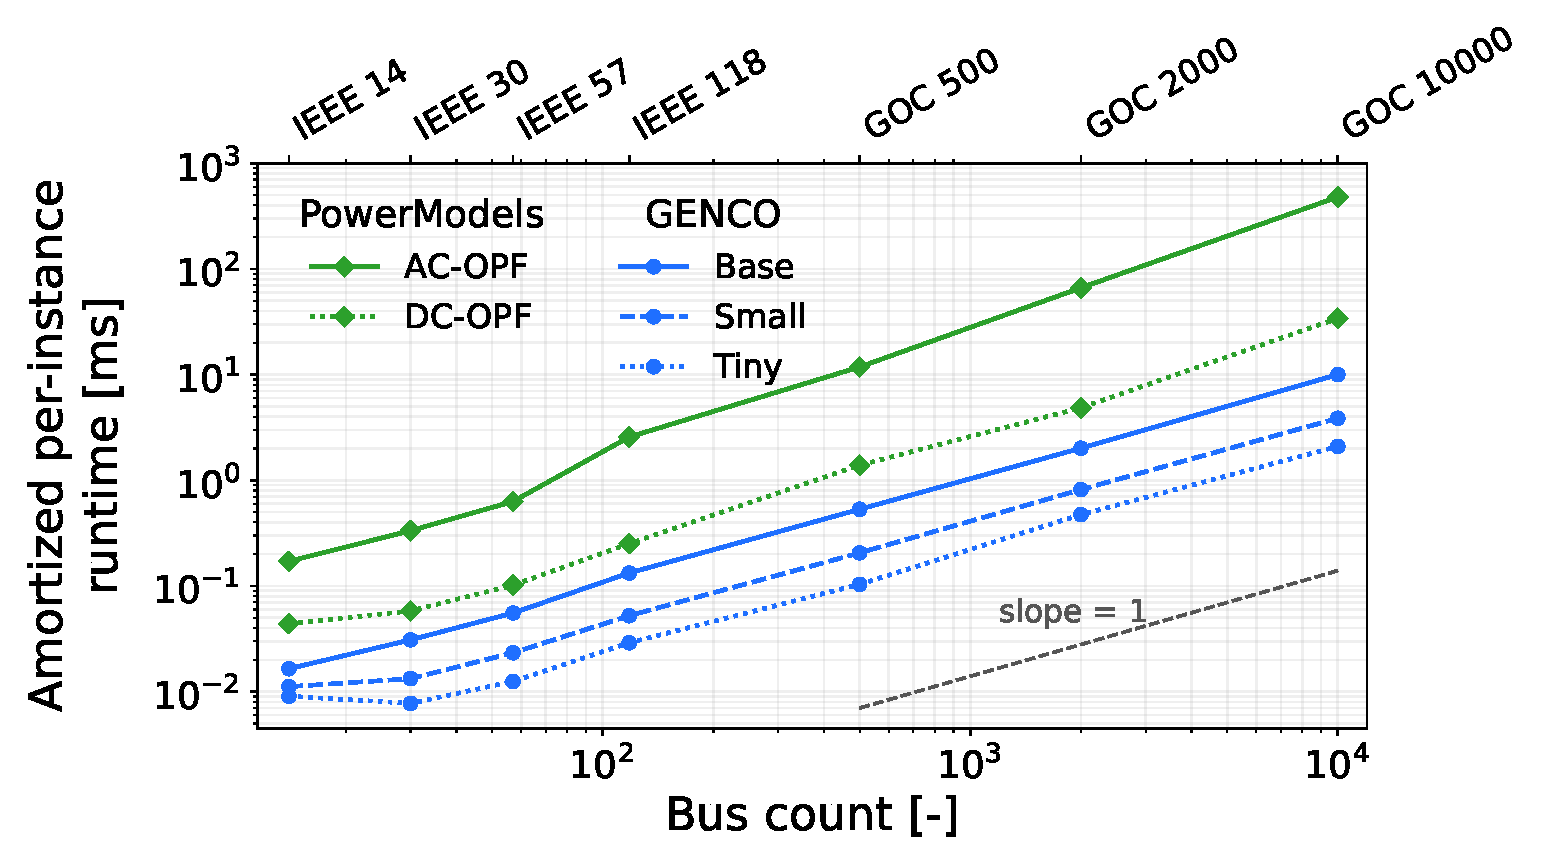
\includegraphics[width=\linewidth]{figures/runtime_analysis/runtime_comparison_from_raw_opf.pdf}
    \caption{Amortized per-instance runtime versus grid size for \genco and PowerModels AC-OPF and DC-OPF solvers. Results are reported for the optimal batch size for \genco and the best worker count for PowerModels. Four-largest-grid scaling exponents are 1.18 for AC-OPF, 1.09 for DC-OPF, and 0.97/0.95/0.94 for \genco Base/Small/Tiny.}
    \label{fig:gridsize_runtime_opf}
\end{figure}



\paragraph{\genco's utility for OPF.} The performance of \genco Small (which offers the best tradeoff between runtime, optimality, and feasibility) across grid sizes is summarized in \cref{tab:opf_selected_genco_tradeoff}. \genco is substantially faster than AC-OPF and DC-OPF on every grid, reaching an $84.5\times$ speedup over AC-OPF on GOC~2,000. It also produces more feasible and cost-effective solutions than DC-OPF, although these gains generally decrease with grid size. Finally, \genco predicts quantities unavailable from DC-OPF, including voltage magnitudes and reactive power setpoints. Overall, \genco offers a compelling alternative to DC-OPF. Detailed optimality and constraint-violation results for \genco Base and Small are reported in \cref{tab:opf_scaling} in the Appendix.\\



\begin{table}
\centering
\scriptsize
\setlength{\tabcolsep}{4pt}
\renewcommand{\arraystretch}{1.2}
% Requires \usepackage{booktabs}.
\begin{tabular}{@{}l c c c c@{}}
\toprule
Grid
& \shortstack{Speedup\\vs AC-OPF}
& \shortstack{Opt. gap reduction\\vs DC-OPF}
& \shortstack{Violation reduction\\vs DC-OPF}
& \shortstack{Speedup\\vs DC-OPF} \\
\midrule
  14 & $16.1\times$ & $55.2\times$ & $86.0\times$ & $4.14\times$ \\
  30 & $22.9\times$ & $31.8\times$ & $72.4\times$ & $3.99\times$ \\
  57 & $26.5\times$ & $6.28\times$ & $4.67\times$ & $4.29\times$ \\
 118 & $48.4\times$ & $2.85\times$ & $2.40\times$ & $4.75\times$ \\
 500 & $54.3\times$ & $3.20\times$ & $10.3\times$ & $6.40\times$ \\
2000 & $84.5\times$ & $1.85\times$ & $6.70\times$ & $6.19\times$ \\
\bottomrule
\end{tabular}
\caption{Performance scaling summary for \genco Small on Optimal Power Flow; Speedups $>$1 mean faster; optimality and feasibility improvements are ratios of DC-OPF to \genco mean metrics.}
\label{tab:opf_selected_genco_tradeoff}
\end{table}



\begin{boxH}
\paragraph{Takeaways.}

\begin{itemize}

% \item We introduced a method to perform a fair run-time assessment with i) fully utilized CPU and GPU, ii) the choice of sufficiently large benchmark scenarios, iii) the definition of the wall-clock time, and iv) the selection of equivalent compute hardware. 

\item For PF, \genco starts providing a valuable alternative to DC-PF for large grids ($\geq$2000 buses) by predicting the full AC operating state, including voltage magnitudes and reactive power, while achieving active power-balance residuals comparable to DC-PF, with up to \maxpfspeedups speedup over Newton--Raphson and only a \dcpfspeedupovergenco runtime relative to DC-PF.

\item For OPF, \genco is compelling across all evaluated grid sizes: Small is $16$--$85\times$ faster than AC-OPF and $4$--$6\times$ faster than DC-OPF, while reducing DC-OPF optimality gaps by $1.9$--$55\times$ and feasibility violations by $2.4$--$86\times$.



\end{itemize}
\end{boxH}



\subsection{Robustness \& Generalization}

\label{subsec:generalization}

A key requirement for any power-system solver is reliable performance across (1) diverse topologies, (2) operating conditions, and (3) network sizes. Classical solvers are well established across these dimensions, with their main limitation being occasional convergence failures in challenging cases~\cite{tostado2021solving}. In contrast, robustness across these dimensions remains a central challenge for neural solvers, which typically require retraining when topology or operating regimes change. Achieving high accuracy across diverse scenarios is therefore essential for the scalability and practical deployment of neural solvers. We evaluate \genco along three axes: generalization to topology perturbations beyond the training distribution (\cref{subsubsec:top_perturbation}), robustness under stressed operating conditions such as thermal overloads and voltage violations (\cref{subsubsec:robustness}), and transfer to previously unseen grids (\cref{subsubsec:transfer}). %We focus on PF, while a similar analysis for OPF is left for future work.



\subsubsection{Generalization to Topology Perturbations}

\label{subsubsec:top_perturbation}

\paragraph{Experiment setup.} \genco is evaluated under contingency levels that match or exceed those seen during training to assess robustness to topology perturbations. Specifically, \genco Base is trained on 140,000 AC-PF samples\footnote{Using \datakit, we generated 200,000 samples, of which 176,415 converged; 80\% of converged samples were used for training.} from the Texas 2000-bus system with up to \textbf{N-2} contingencies, corresponding to the removal of up to two branches and/or generators. The test set contains 9,000 cases for each contingency level from N-1 to N-20. Components are removed uniformly across the grid, and islanding cases are filtered out. Since perturbations are applied after computing the base dispatch (\cref{subsubsec:gen_setpoints}), the resulting operating points may exhibit voltage violations, branch overloads, large angle differences, and reactive-power limit violations.






\begin{figure}
\centering
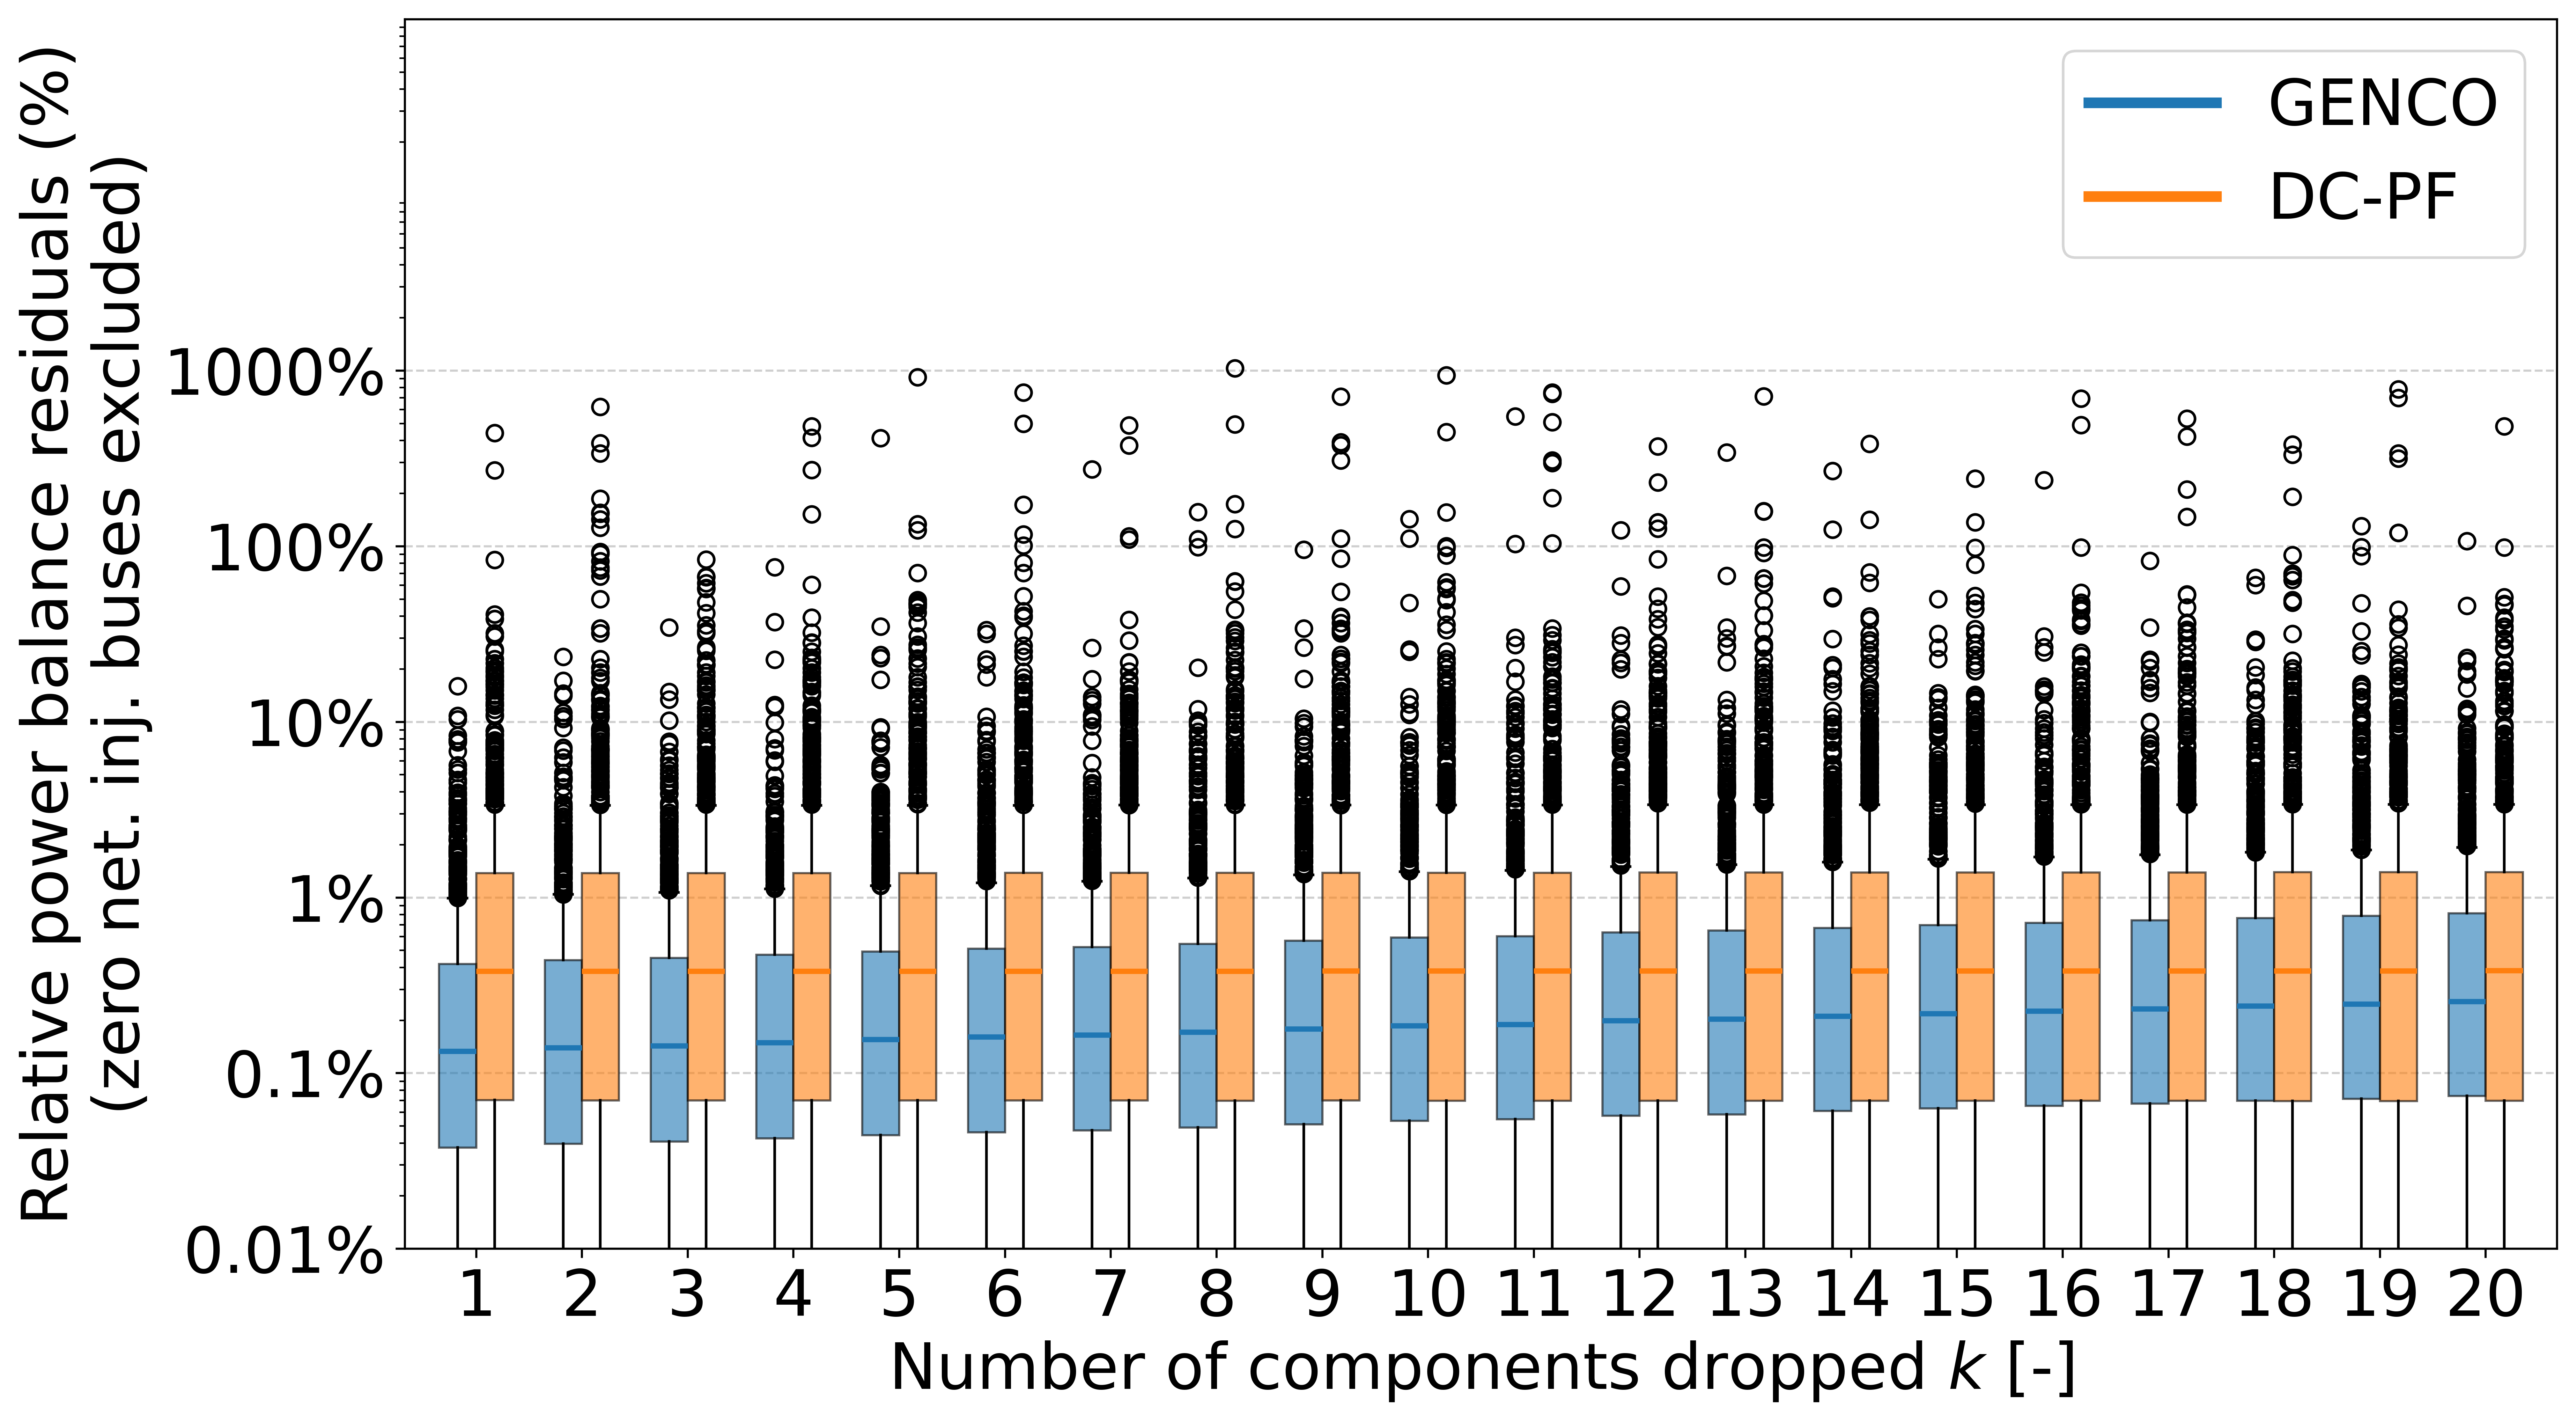
\includegraphics[width=\linewidth]{figures/robustness/boxplot_relative_residuals.png}
\caption{Bus-level active power-balance residuals (excluding zero net injection buses) for \genco and DC-PF under N-$k$ contingencies ($k=1,\dots,20$) on the Texas 2000-bus system. \genco is trained only on N-2 perturbations. Whiskers indicate 1.5$\times$IQR.}
\label{fig:performance_k_1_20}
\end{figure}

\paragraph{Results.} We evaluate bus-level relative active power-balance residuals, as opposed to absolute residuals, which mask large errors at low-injection buses. The bus-level relative active power-balance residuals are defined as the active power-balance residuals divided by the magnitude of the net bus injection\footnote{We filter out buses with zero net injection for which such a metric cannot be computed. These represent ~25\% of all buses across the entire dataset, and we report absolute metrics separately for them in \cref{appendix:zeroinj}}. This normalization approach makes the metric comparable across buses with vastly different injection levels. \genco consistently outperforms DC-PF across all contingency levels, including those beyond the training distribution, i.e., for N-k with $k > 2$ (\cref{fig:performance_k_1_20}). Residuals increase with outage count, but degradation remains gradual: \genco achieves 2.85$\times$ lower median residuals than DC-PF for N-1 contingencies and 1.5$\times$ lower median residuals for N-20.\\


Outlier residuals displayed in \cref{fig:performance_k_1_20} are high for both DC-PF and \genco (between 9.2 and 9.8 percent of the buses across all contingency orders and solvers). Thus, we report the fraction of buses with residuals below practically relevant thresholds for $k=10$ in \cref{fig:threshold_share_relative_k10}: \genco outperforms DC-PF at all levels, including 1\% (83.65\% vs 69.30\%). The same trend holds for absolute thresholds (\cref{fig:abs_threshold_k10}, \cref{appendix:top}), e.g., at 1~MW (97.69\% vs 85.78\%). Further details about the 1\% threshold fraction across contingencies can be found in \cref{fig:rel_threshold_vs_k} in \cref{appendix:top}.


\begin{figure}
\centering
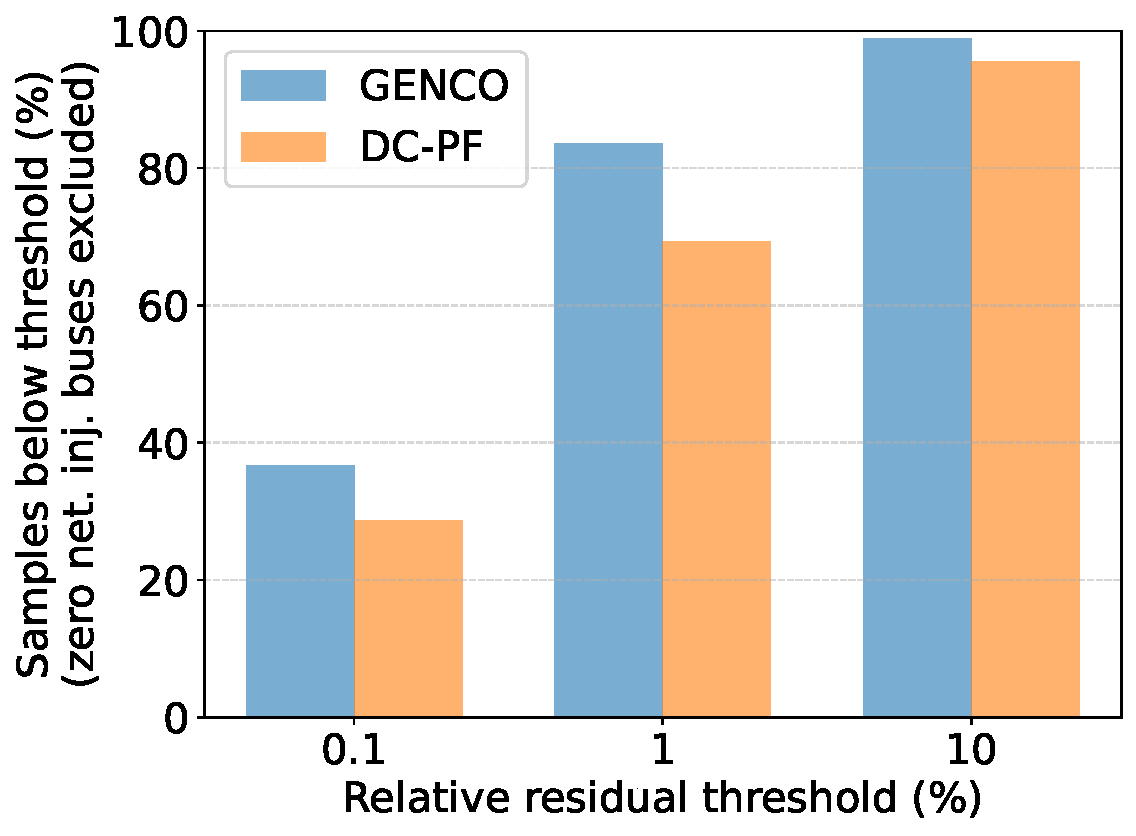
\includegraphics[width=0.7\linewidth]{figures/robustness/threshold_share_relative_k10.pdf}
\caption{Percentage of samples below relative active power-balance residual thresholds at $k=10$ (excluding zero net injection buses). \genco achieves a larger share of low-residual predictions than DC-PF across all reported thresholds.}
\label{fig:threshold_share_relative_k10}
\end{figure}




\subsubsection{Robustness to Out-of-Operating-Limit Scenarios}
\label{subsubsec:robustness}

\paragraph{Experiment setup.} Next, we evaluate GENCO's performance on operating points that violate thermal or voltage limits. These out-of-operating-limit elements are rare: only $0.0071$\% of branches are overloaded, corresponding to 1,979 out of a total of 28,052,640 branches in the dataset. Thus, such cases are underrepresented during model training relative to branches operating within nominal limits. For this experiment, we use the same \genco Base model as in the previous experiment, trained and tested on the N-2 contingency dataset.

\paragraph{Results.} The comparison of \genco and DC-PF branch loading predictions against AC-PF is depicted in \cref{fig:dc_loading}. Branch loadings are normalized by their thermal limits, such that values above 1.0 correspond to overloads. While DC-PF exhibits substantial dispersion, \genco remains closely aligned with the diagonal across both normal and overloaded operating regimes, as quantified by the coefficient of determination.\\

To further assess performance near and beyond thermal limits, \cref{fig:loading_boxplot} reports absolute loading errors as a function of the true loading level. \genco consistently outperforms DC-PF across all loading bins, including overload conditions that are strongly underrepresented in the training data. For lines with true loadings between 1.0 and 1.1, \genco achieves a mean absolute error of 0.004, enabling accurate identification of overloaded components. \\

Since DC-PF does not predict voltage magnitudes, voltage-related results are reported separately in \cref{appendix:voltage_violations}. There, we show that \genco accurately captures both normal and out-of-limit voltage regimes despite the scarcity of voltage violations in the training data. These results indicate that explicit oversampling of out-of-limit operating points is not required for accurate overload prediction.\\


\begin{figure}
\centering
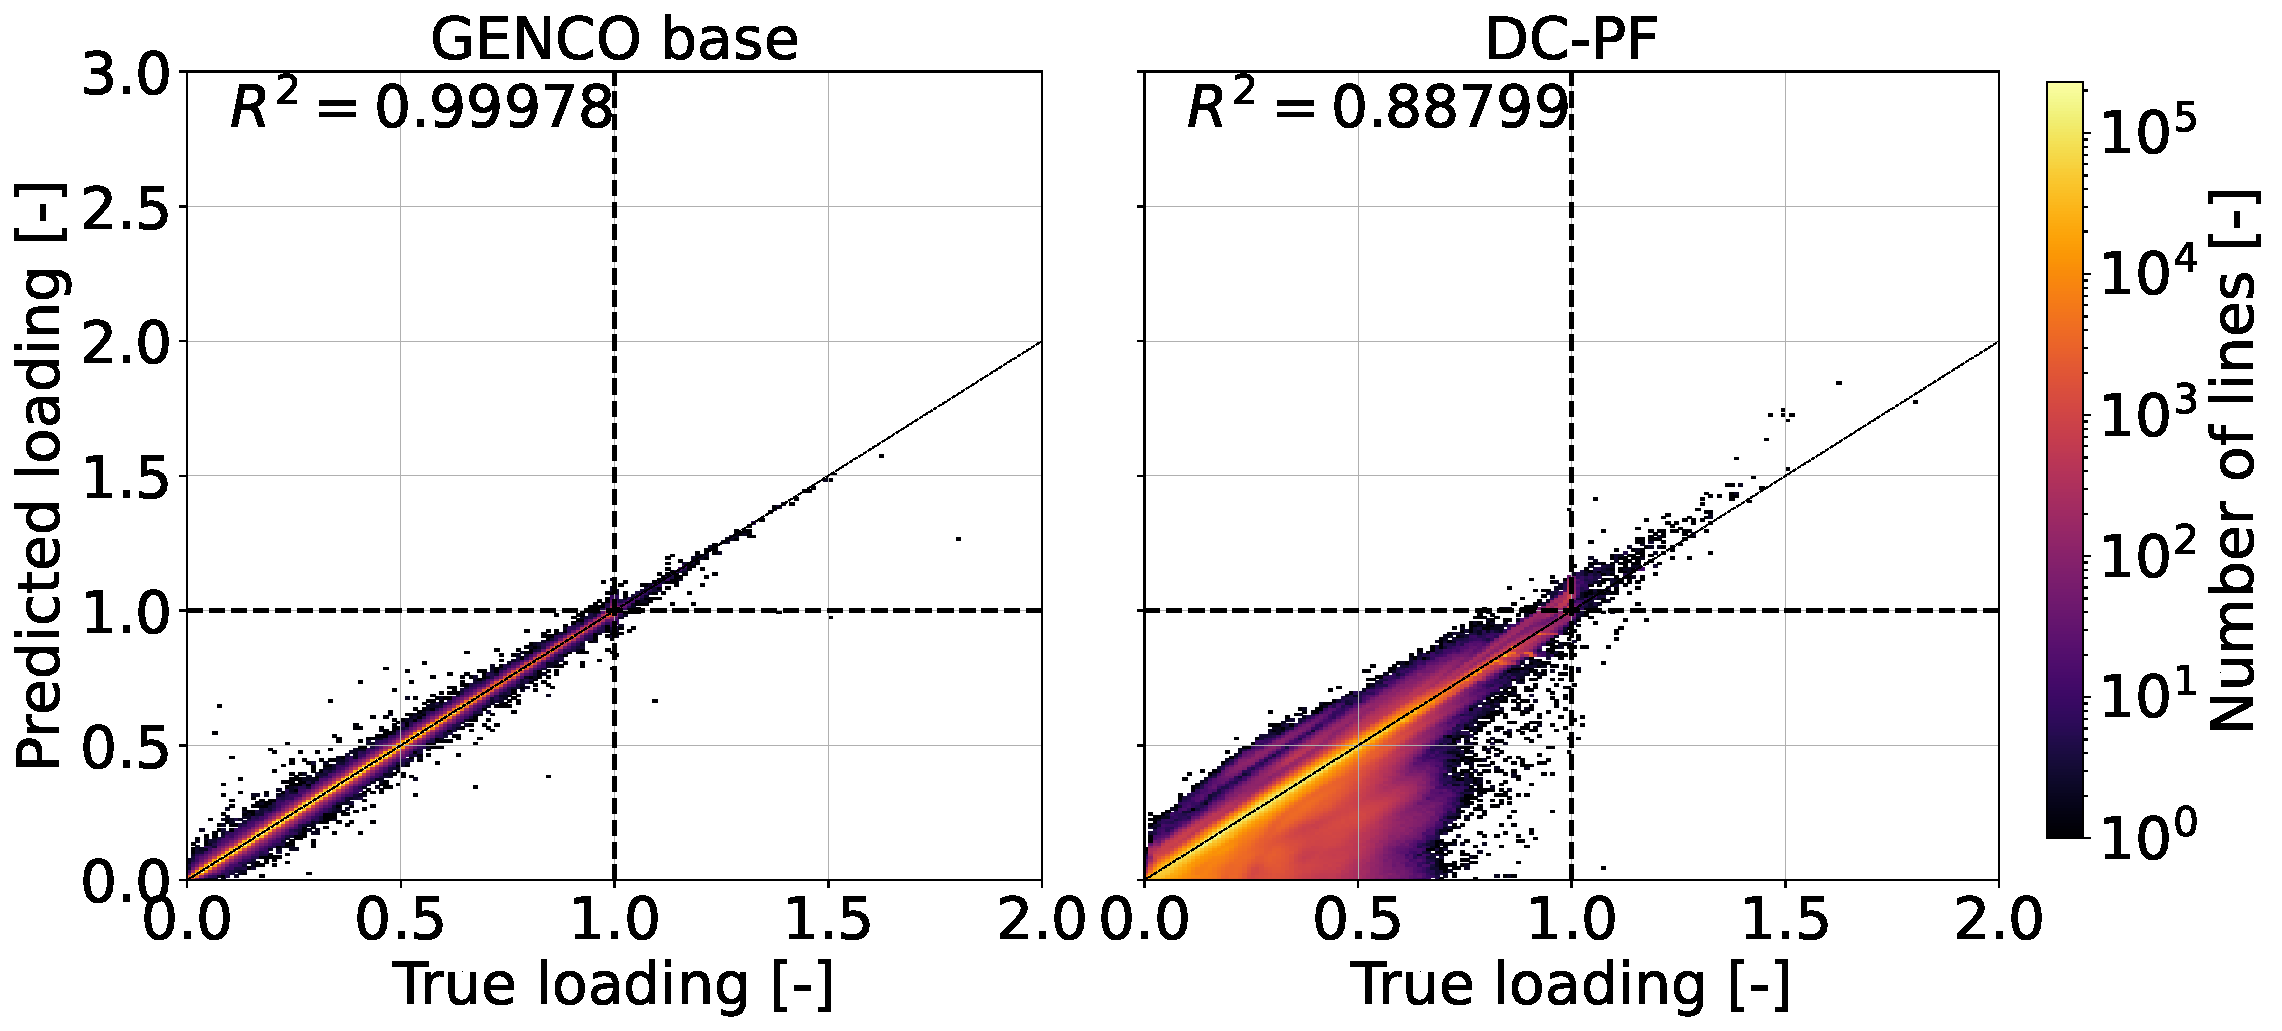
\includegraphics[width=0.9\linewidth]{figures/robustness/mass_correlation_density_Texas_vs_dc.pdf}
\caption{Relative branch loading predictions obtained with \genco base (left) and DC-PF (right) compared to AC-PF loadings. Values above 1.0 indicate thermal overloads.}
\label{fig:dc_loading}
\end{figure}









\begin{figure}
\centering
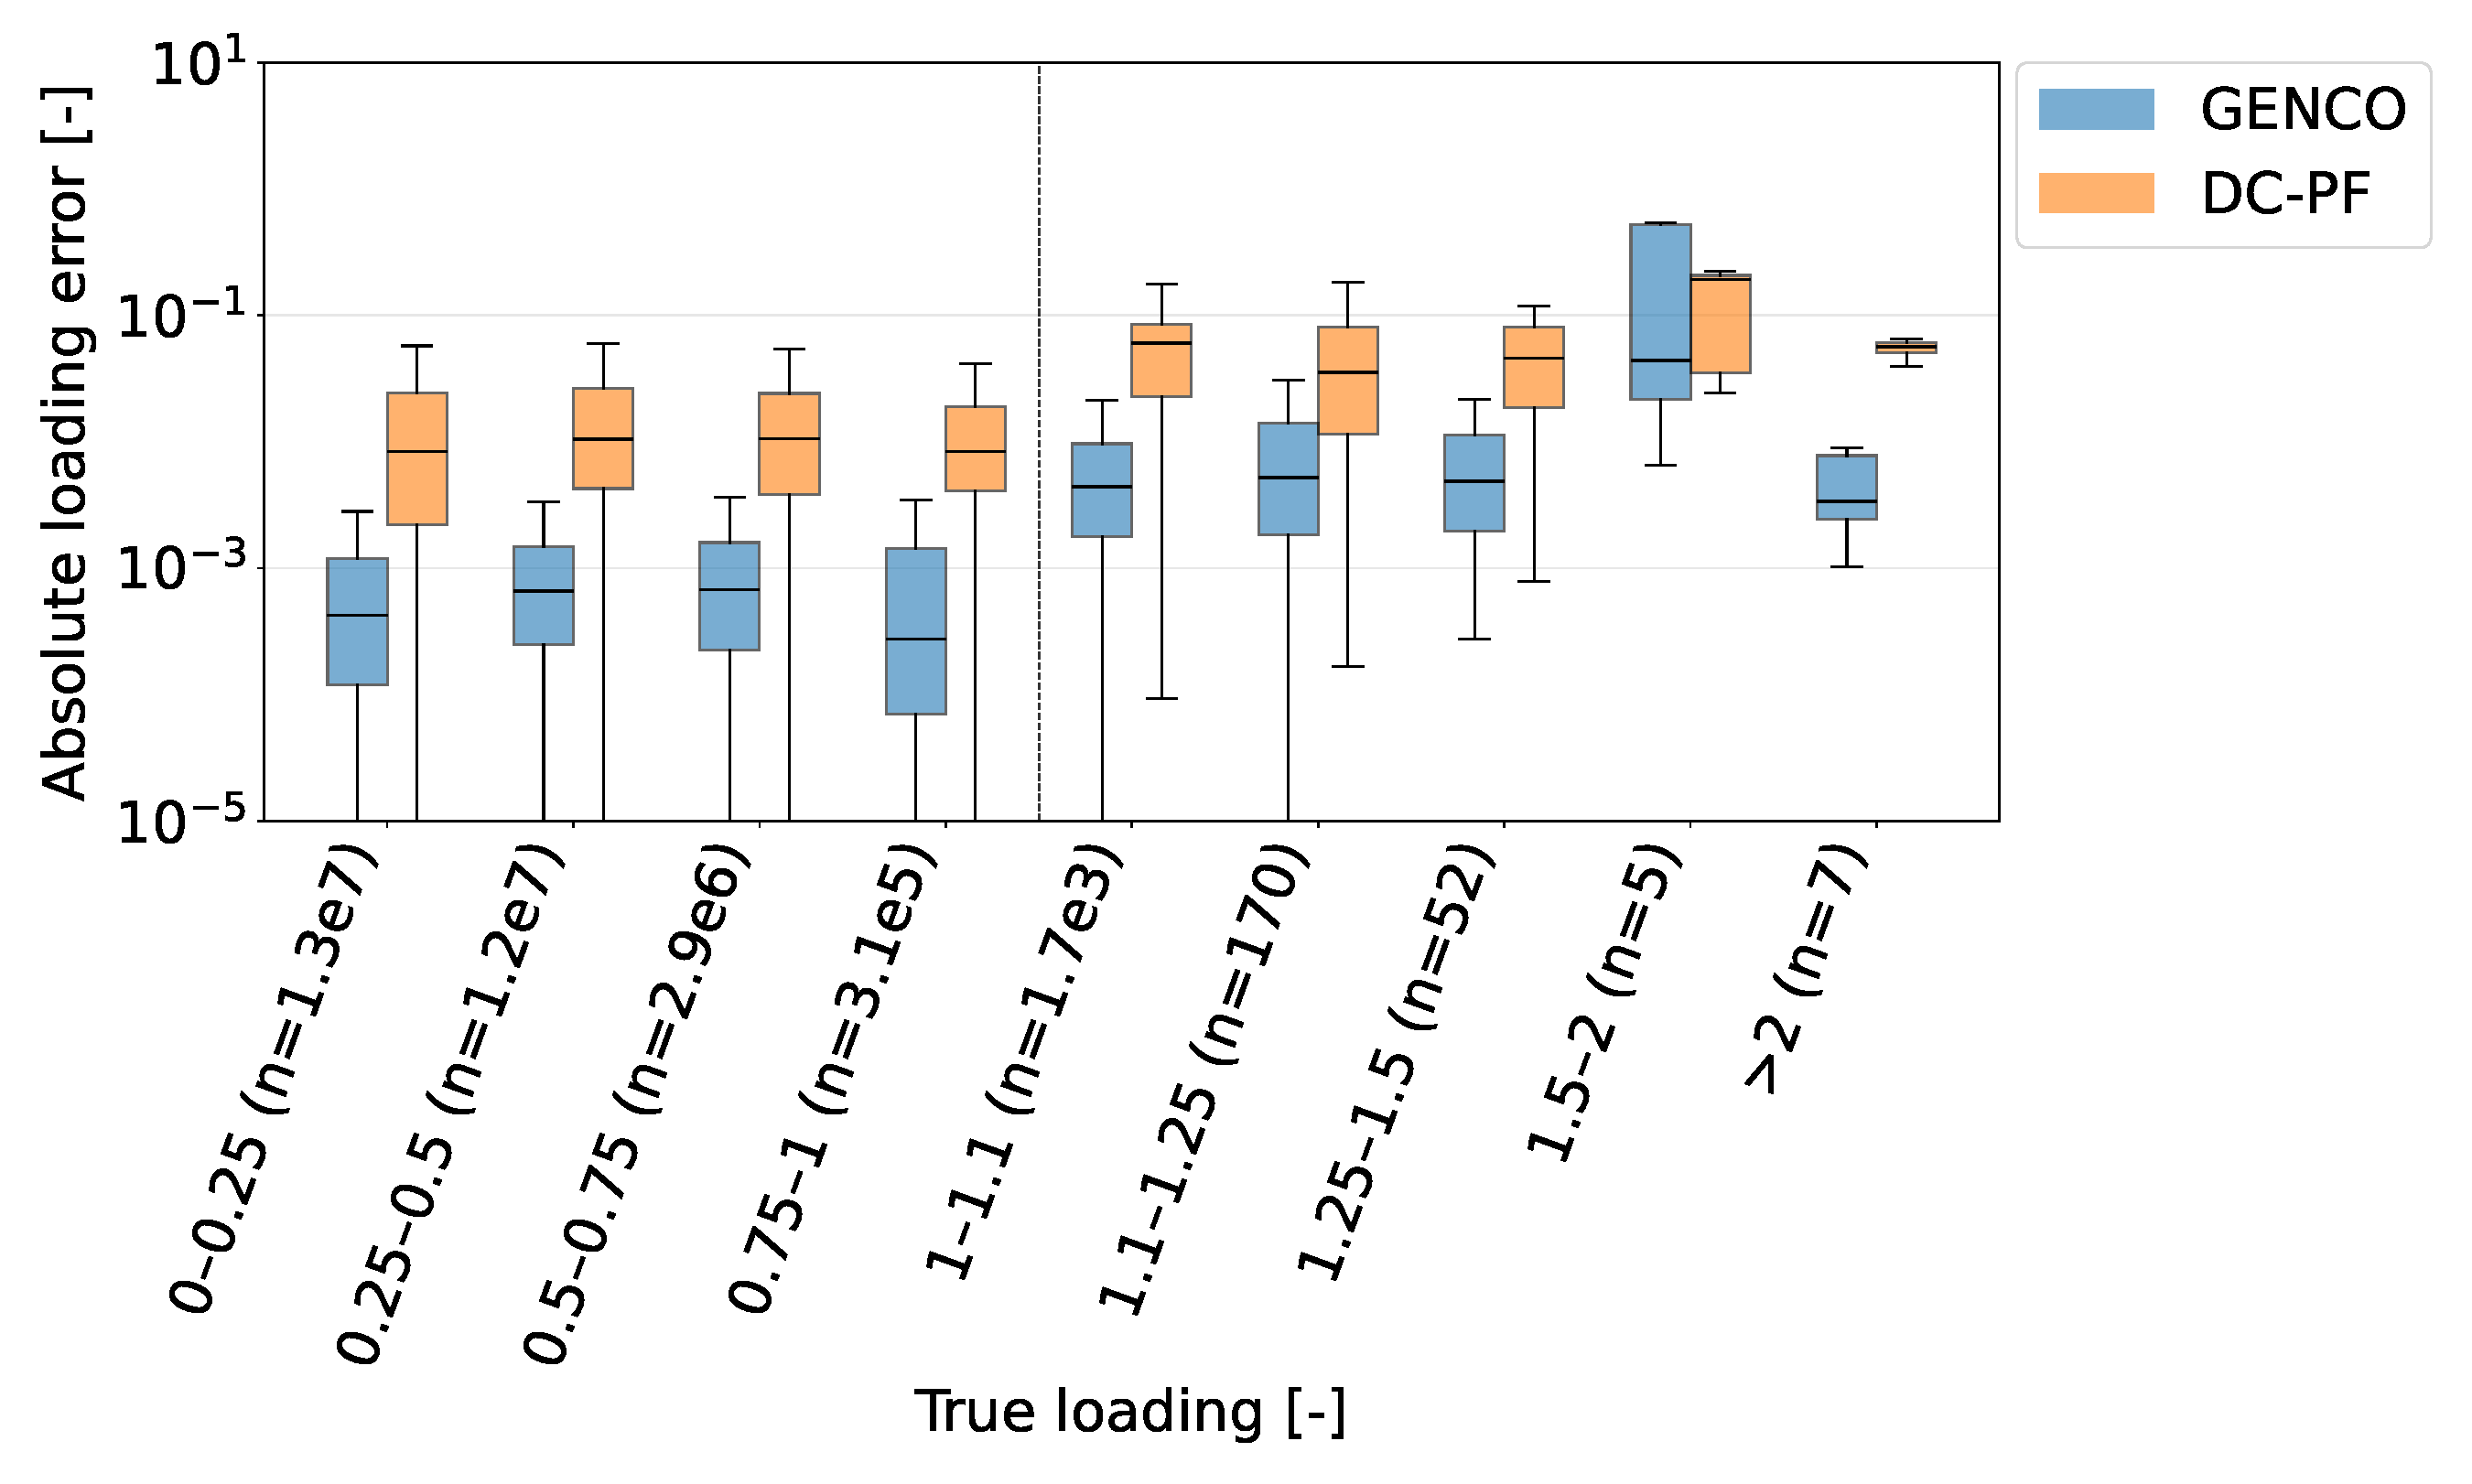
\includegraphics[width=0.9\linewidth]{figures/robustness/loading_error_boxplot_by_true_loading_Texas.pdf}
\caption{Absolute branch loading prediction error as a function of the true loading level. $n$ indicates the number of test samples in each bin.}
\label{fig:loading_boxplot}
\end{figure}





\subsubsection{Transfer to Unseen Grids and Data Efficiency}
\label{subsubsec:transfer}
\begin{figure} 
\centering 
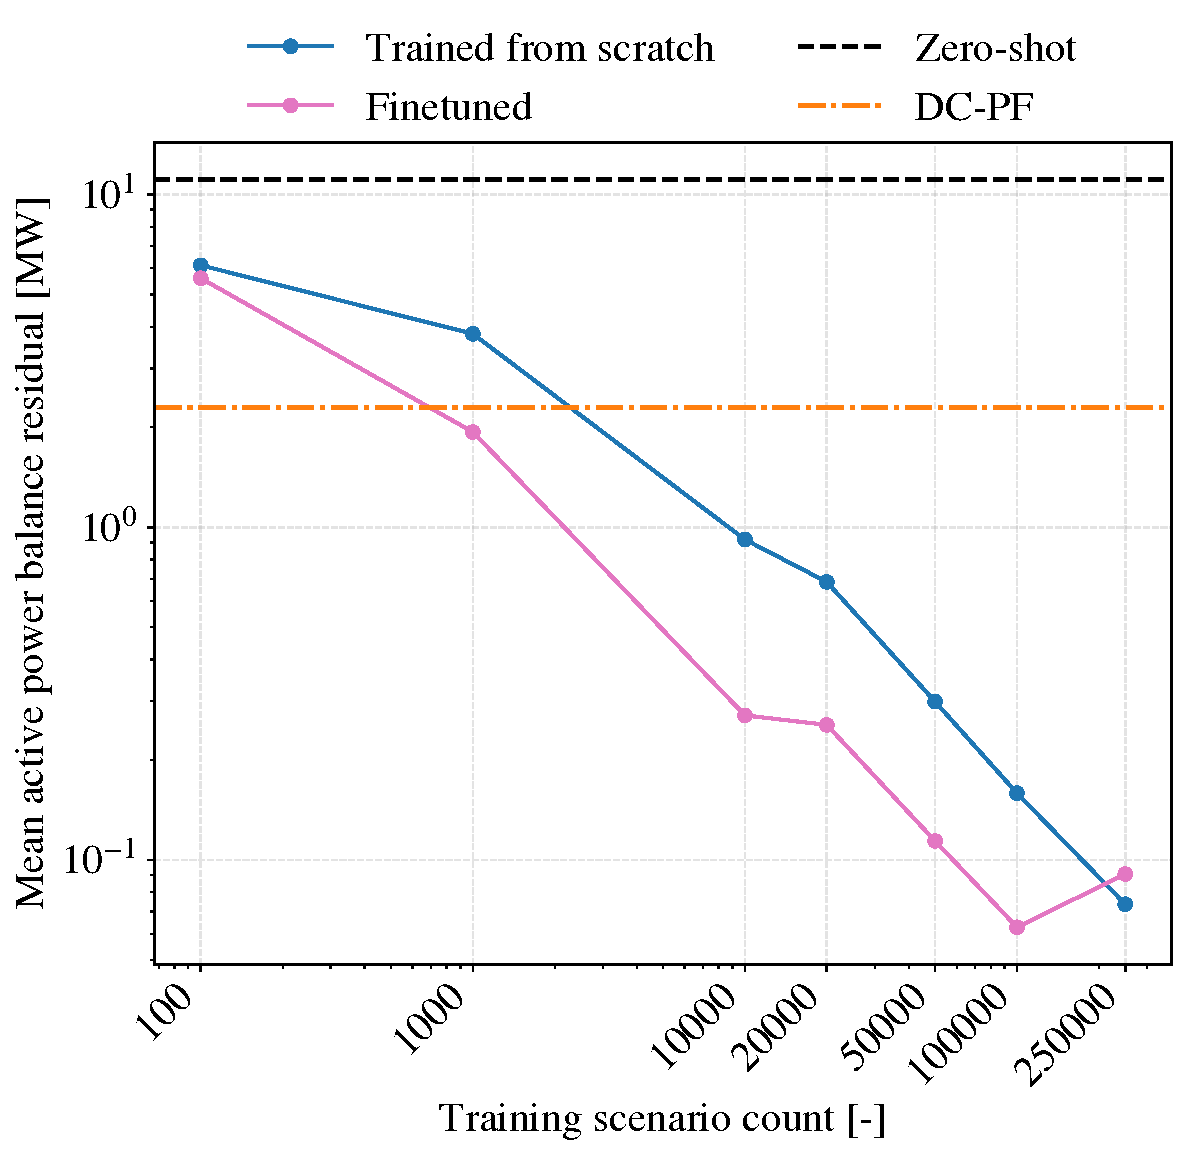
\includegraphics[width=0.85\linewidth]{figures/robustness/scratch_vs_finetune_active_residuals.pdf} 
\caption{Mean active power-balance residuals on IEEE 118 for fine-tuned pretrained models and models trained from scratch using datasets of varying size. DC-PF and the zero-shot pretrained model (without fine-tuning) are shown as baselines.} 
\label{fig:transfer} 
\end{figure}

An important objective for neural PF solvers is rapid adaptation to entirely new grids using only a limited number of grid-specific samples. This capability would reduce deployment costs, since acquiring AC-PF datasets and training neural solvers from scratch for every new topology is time-consuming and expensive. We therefore investigate the transferability of pretrained \genco models to unseen grids under different levels of fine-tuning. To increase topology diversity during pretraining, we generate subgrids from existing grids and evaluate transfer to unseen topologies.

\paragraph{Experiment setup.}
Only around 50 different grids for which PF converges are available in PGLib. To increase the number of pretraining topologies, we extract subgrids from base grids using Metropolis-Hastings random walks. Power flows on cut lines are aggregated into dummy generators or loads depending on their sign. Using this approach, we generate 100 subgrids from 10 PGLib base cases, with sizes ranging from 100 to 1000 buses. We generate 9,000 PF samples per subgrid using \datakit, yielding 900,000 scenarios. Validation is performed on 10 unseen subgrids. \\ 

We then fine-tune the pretrained GENCO model on the IEEE 118-bus system using varying numbers of grid-specific samples. The resulting fine-tuned models are compared with models trained from scratch using the same datasets\footnote{The only difference between the two models is their weight initialization: the fine-tuned model starts from pretrained weights, whereas the scratch model uses random initialization.}.

\paragraph{Results.}
The active power-balance residuals are shown in \cref{fig:transfer}, together with those obtained with DC-PF and with the pretrained GENCO used in a zero-shot manner, i.e., without any fine-tuning on the test grid. The pretrained model has poor zero-shot generalization, with an average residual of 11.07 MW compared with 2.30 MW for DC-PF. However, with only 1,000 grid-specific samples, fine-tuning already outperforms DC-PF (1.93 MW), whereas training from scratch remains worse (3.81 MW). With 10,000 samples, fine-tuning further reduces the residual to 0.27 MW, compared with 0.92 MW when training from scratch. At 250,000 samples, scratch training surpasses fine-tuning, which slightly degrades under extensive fine-tuning.\\

Overall, these results show that topology-diverse pretraining can accelerate adaptation to unseen grids when grid-specific data are limited. However, with sufficient data from a single grid, training from scratch can eventually outperform pretraining. Further work is needed to reduce the number of fine-tuning samples required for true few-shot adaptation.\\




\begin{boxH}
\paragraph{Takeaways.}

\begin{itemize}

\item \genco generalizes to contingency levels up to N-20 despite training only on N-2, achieving 2.85$\times$ lower median residuals than DC-PF for N-1 contingencies and 1.5$\times$ lower median residuals for N-20.

\item \genco remains robust under out-of-operating-limit scenarios despite training on fewer than $0.01$\% such out-of-limit elements, outperforming DC-PF for line-loading prediction and detecting voltage violations beyond the capabilities of DC-PF.

\item A pretrained \genco transfers effectively to new grids, with only 1,000 grid-specific samples sufficient to outperform DC-PF on IEEE 118, although zero-shot generalization remains an open challenge.

\end{itemize}
\end{boxH}




\subsection{Validation on Real Data from the Hydro-Québec Grid}
\label{subsec:hq1200}

Finally, we evaluate \genco on the real Hydro-Qu\'ebec HQ1200 transmission network, extending the validation beyond the synthetic IEEE/GOC topologies. All experiments are done for the PF task. HQ1200 comprises 1,200 buses and differs markedly from these benchmarks through its V-shaped topology, with long corridors linking northern generation to southern load. These long-range dependencies make HQ1200 a non-trivial test for \genco.\\

As we only have a limited amount of SCADA data samples---roughly one year of measurements at 30-minute resolution---we proceed in two stages.
First, we pretrain \genco on synthetic HQ1200 operating points generated with \datakit (\cref{subsec:comparison_data_hq}), and compare \genco's performance against GRIT-HQ and classical AC/DC power flow solvers (\cref{subsubsec:hq_synthetic}).
Second, we fine-tune the pretrained \genco model on varying amounts of SCADA scenarios, and compare against \genco trained from scratch, on the same SCADA splits (\cref{subsubsec:hq_scada}).

\subsubsection{Pretraining on synthetic data}
\label{subsubsec:hq_synthetic}

First, we compare \genco Tiny against Hydro-Qu\'ebec Research Institute's GRIT-HQ model. Unlike the more general-purpose \genco architecture, GRIT-HQ is specialized for power flow on bus-level graphs. It is based on the GRIT architecture~\cite{ma2023graph}, uses random-walk structural encodings, and scales linearly with graph size; details are given in \cref{appendix:hqgrit}. Both models are trained on 200{,}000 synthetic HQ1200 samples (80/10/10 train/validation/test), with three independent seeds.\\

Mean active and reactive power-balance residuals are reported in \cref{tab:hq1200_results}. GRIT-HQ exhibits higher active power-balance residuals than DC-PF, whereas \genco reduces active power-balance residuals by approximately $2.5\times$ relative to DC-PF and substantially improves reactive power-balance residuals compared with GRIT-HQ. The resulting residual magnitudes of \genco are small compared to balancing and remedial actions routinely deployed by Hydro-Québec~\cite{EU2017_2195,EU2017_1485_SOGL}. This result is also consistent with IEEE grids of comparable size (\cref{fig:gridsize_vs_residuals_pf}), indicating robustness to a markedly different topology without architectural changes.

\begin{table}\centering\small
\resizebox{0.8\columnwidth}{!}{%
\renewcommand{\arraystretch}{1.2}
\begin{tabular}{c|c|c} \hline
    \multicolumn{1}{c|}{\textbf{Model}} &
    \multicolumn{2}{c}{\textbf{Power Balance Residual}} \\ \hline
    &
    \textbf{Active [MW]} &
    \textbf{Reactive [MVar]} \\ \hline
    \textbf{\genco Tiny}
    & \textbf{1.1 \scriptsize $\pm$ 0.3}
    & \textbf{0.5 \scriptsize $\pm$ 0.2} \\
    GRIT-HQ
    & 3.87 \scriptsize $\pm$ 0.02
    & 4.03 \scriptsize $\pm$ 0.44 \\
    DC-PF
    & 2.89
    & --- \\
    \rowcolor[gray]{0.92}
    AC-PF
    & 2.94e-9
    & 1.81e-9 \\ \hline
\end{tabular}}
\caption{Mean active and reactive power-balance residuals on the synthetic HQ1200 dataset.
Errors denote standard deviation over three seeds.
Bold values indicate the best learning-based method.}
\label{tab:hq1200_results}
\end{table}

\subsubsection{Fine-tuning on real SCADA data}
\label{subsubsec:hq_scada}

Next, we explore whether \genco can perform well on real HQ data under limited training on SCADA data.
Starting from the HQ1200 pretrained checkpoint of \cref{subsubsec:hq_synthetic}, we fine-tune on real SCADA scenarios using $N\in\{100,10^3,10^4,1.5\times10^4\}$ labeled training samples, and compare against \genco solvers trained from scratch on the same training samples. For the evaluation, we use a held-out set of 1{,}702 SCADA samples. In addition, we report the zero-shot performance of the pretrained \genco model, without SCADA fine-tuning, as well as the performance of DC-PF on the same evaluation set. All settings are repeated over three seeds; we report mean active power-balance residuals with sample standard deviation.\\

\cref{fig:hq_scada_finetune} shows active power-balance residuals versus the number of SCADA training scenarios. Zero-shot transfer remains poor, indicating that synthetic pretraining alone is insufficient for the model to perform well on real SCADA data. Fine-tuning rapidly closes this gap: with 15,000 training samples, fine-tuning achieves $3.36\pm0.05$~MW, an order of magnitude below training from scratch ($21.1\pm8.4$~MW) and approaching the DC-PF residual of $2.90$~MW on the same evaluation set. We note that the continued improvement with increasing amounts of SCADA samples also suggests that further real-data fine-tuning could close the remaining gap. Training from scratch also exhibits substantially higher variance at low sample counts. These results show that synthetic pretraining on HQ1200 enables data-efficient adaptation of \genco to real SCADA measurements.\\

\begin{figure}
\centering
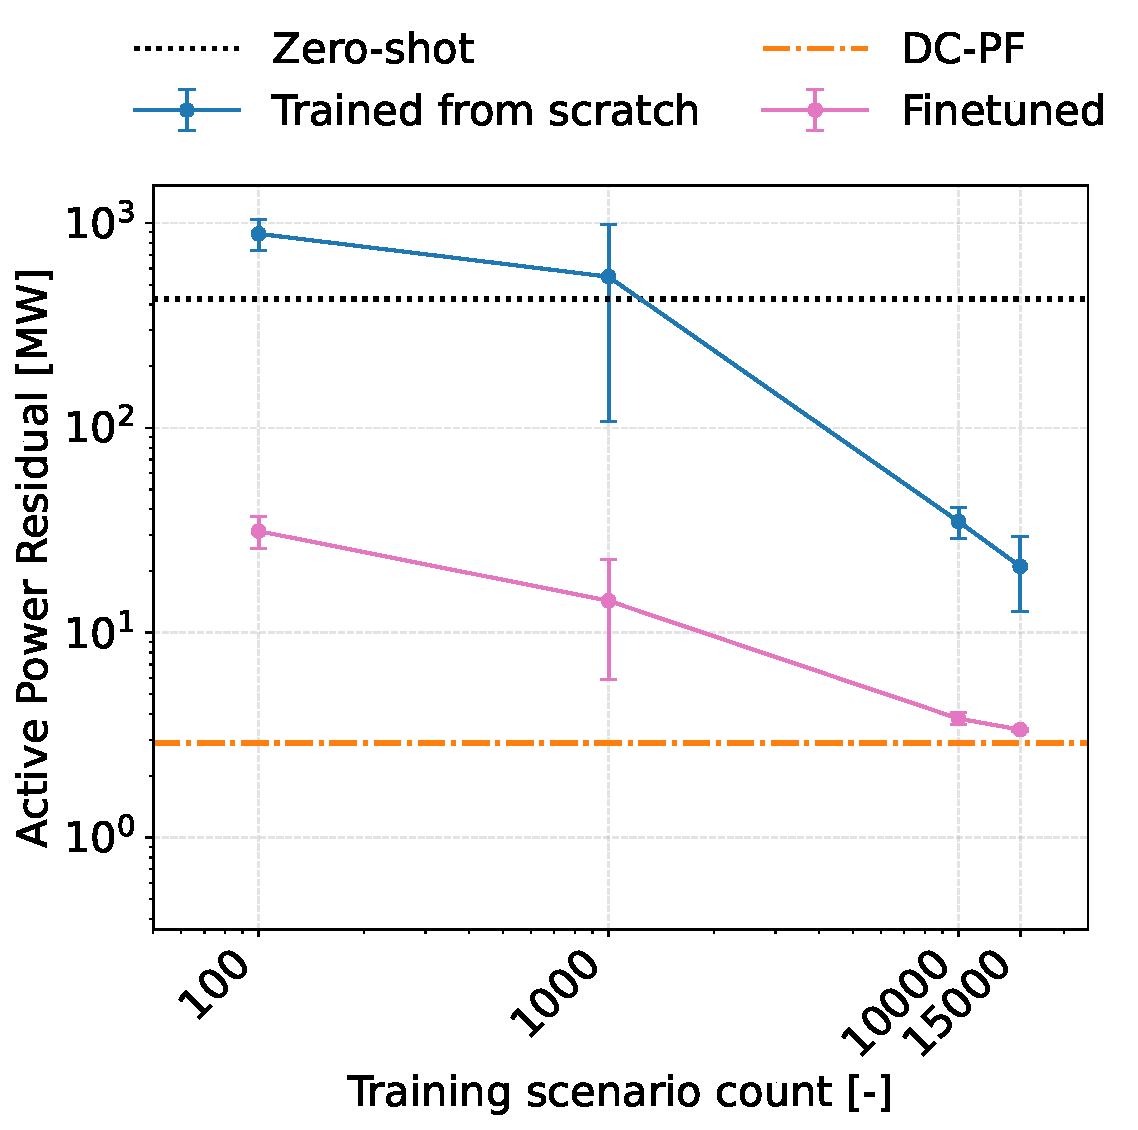
\includegraphics[width=0.85\columnwidth]{figures/hq/hq_scratch_vs_finetune_active_residuals.pdf}
\caption{Mean active power-balance residuals on HQ SCADA versus number of training scenarios, comparing fine-tuning of the synthetically pretrained model against training from scratch (mean $\pm$ sample std over three seeds).
The dotted line denotes zero-shot performance of the pretrained model.}
\label{fig:hq_scada_finetune}
\end{figure}

\begin{boxH}
\paragraph{Takeaways.}
\begin{itemize}
\item \genco successfully transfers to a real grid and is evaluated on real SCADA data: after fine-tuning on 15,000 Hydro-Québec SCADA samples, it achieves a mean active power-balance residual close to that of DC-PF ($3.36$~MW vs. $2.90$~MW).
\item Pretraining on synthetic HQ1200 scenarios generated with \datakit enables substantially more data-efficient adaptation to real SCADA measurements, reducing the residual by an order of magnitude relative to training from scratch with the same 15,000 SCADA samples.
\end{itemize}
\end{boxH}

